\documentclass{sig-alternate-10pt}

\usepackage[hyphens]{url}
\usepackage{bold-extra}
\usepackage{color}
\usepackage{courier}
\usepackage{enumitem}
\usepackage{etoolbox}
\usepackage{hyperref}
\usepackage{listings}
\usepackage{subcaption}

\lstset{
  showspaces=false,
  showtabs=false,
  breaklines=true,
  showstringspaces=false,
  breakatwhitespace=true,
  escapeinside={(*@}{@*)},
  basicstyle=\footnotesize\ttfamily,
  columns=fullflexible
}

\def\Snospace~{\S{}}
\renewcommand*\sectionautorefname{\Snospace}
\renewcommand*\subsectionautorefname{\Snospace}
\renewcommand*\subsubsectionautorefname{\Snospace}
\renewcommand*{\figureautorefname}{Fig.}

\begin{document}

\newcommand{\sysname}{AdaptiveStream}
\newcommand{\para}[1]{\medskip\noindent\textbf{#1}}
\newcommand{\paraf}[1]{\smallskip\noindent\textbf{#1}}
\newcommand{\todo}[1]{{\color{ACMRed}\bf{TODO: #1}\normalfont}}.

%%% Local Variables:
%%% mode: latex
%%% TeX-master: "sosp17"
%%% End:


% \conferenceinfo{WOODSTOCK}{'97 El Paso, Texas USA}
% \CopyrightYear{2007}
% \crdata{0-12345-67-8/90/01}
% --- End of Author Metadata ---

\title{Adaptive Stream Processing in Wide-Area Network}

\numberofauthors{1}
\author{ \alignauthor \textit{Anonymous for submission} }

\maketitle

\begin{abstract}
  In this paper, we present \sysname{}, a stream processing system that adapts
  the application execution to wide-area network changes. \sysname{} enables
  graceful degradation during resource fluctuations: trading application
  accuracy for the freshness of analytics. To achieve this, \sysname{} explores
  the PAR (performance-accuracy-resource) principle. We employ an offline
  profiling process that explores the parameter space of each application and
  generates a profile of the application. During runtime, the system would alter
  the application execution if the resource level changes. We evaluate
  \sysname{} against three real-world applications: large-scale IoT
  applications, video analytics and distributed CDN monitoring. At places where
  traditional approaches would lead to either significant application accuracy
  drop or long tail, our system gracefully handles the application.
\end{abstract}

% \category{H.4}{Information Systems Applications}{Miscellaneous}
% \terms{Theory}
% \keywords{ACM proceedings, \LaTeX, text tagging}

\section{Introduction}

In this paper, we study streaming analytics in the wide area. Although recent
stream processing systems (such as Storm~\cite{toshniwal2014storm}, Spark
Streaming~\cite{zaharia2013discretized}) can handle large streams of data in a
single cluster, they are not designed to work in the wide area where the
bandwidth is not sufficient to backhaul all the data to a central location.

With the emerging class of Internet of Things (IoT) applications, such as video
surveillance and industrial monitoring, huge data volumes of data are generated
at the edge. In contrast, the Internet's available bandwidth is scarce and
varying, making it impossible to back-haul all the data. And the demand is
growing faster than the network capacity.

When the network resources become insufficient, applications have to choose
between data freshness and data fidelity. Applications based on TCP ensures a
reliable delivery of the data but the backlogged data will increase application
latency. Applications based on UDP could minimize latency by sending packets as
fast as possible, the uncontrolled packet loss along the network may devastate
the application. Either option is not ideal for many streaming anlaytics.

Previous work (JetStream~\cite{rabkin2014aggregation}) has explored the
direction of reducing application's demand with degradation, but it relies on
developers' manual policy, which lacks precision and faces scalability issue.
There are also application-specific optimizations; but they do not
generalize. For example, adaptive video streaming~\cite{yin2015control} is a
well-studied topic but many adaptations aim at human consumption, focusing on
Quality of Experience (QoE). This limits the adaptation space e.g. maintain
25FPS.

Making degradation practical and general across applications is challenging. The
goal is to maximizing application accuracy under the constrain of available
bandwidth with minimal developers' effort (with exhausting). It calls for the
right level of abstraction with a system-level approach.

In this work, we present \sysname{}, which aims to empower developers with an
easy-to-use framework for wide-area streaming analytics. We focus on the scarce
and variable bandwidth and solve it with three ideas: (1) a novel set of APIs
for structured adaptation; (2) a combination of offline and online profiling to
construct a Pareto-optimal strategy; (3) a rate-based congestion control for
runtime adaptation.

Our proposed API imposes a structure on the adaptation that each application can
perform; although the API is narrow, when combined with other operators, we find
the framework is expressive enough for many streaming analytics.

To liberate developers from specifying rules manually, our system employs a
data-driven empirical-analysis approach. The profiling is done both offline and
online. Offline profiling offers bootstrap information that makes online
profiling more efficient. Online profiling alleviates the problem of
\textit{model drift}.

The runtime adaptation automatically adjusts the applications' execution such
that the streaming demand matches the available bandwidth. We employs a
congestion-based congestion control scheme by measuring the bottleneck
bandwidth; in steady state, the system probes for more available bandwidth.

Using \sysname{}, we've built three applications: pedestrian detection,
augmented reality and distributed top-k. We use real-world data for these
applications to evaluate our systems.

The evaluation shows the generated profile for the three applications. Then for
each application, We show how they adapt the behavior at runtime. Under a
controlled experiment, even with only transient network capacity drop, our
system is able to maintain an end-to-end delay for 1 seconds in the wide-area
and accuracy level above 80\%. Application-agnostic protocols creates
significant backlogged data (TCP for about 100 seconds) or unusable accuracy
(UDP).

In summary, this paper makes the following contributions:

\begin{itemize}[leftmargin=16pt]
\item We study in depth of wide-area streaming applications in the case of
  network resource variation.
\item We propose a novel set of APIs to allow for structured adaptation: they
  require minimal developer efforts while being precise with automatic
  profiling.
\item We propose a new congestion control scheme that adapts the application
  data to available bandwidth, with a goal of minimizing the latency.
\item We implement a prototype system.
\item We build three real-world applications and evaluate their behavior
  under different scenarios.
\end{itemize}

%%% Local Variables:
%%% mode: latex
%%% TeX-master: "sosp17"
%%% End:

\begin{figure}
  \centering
  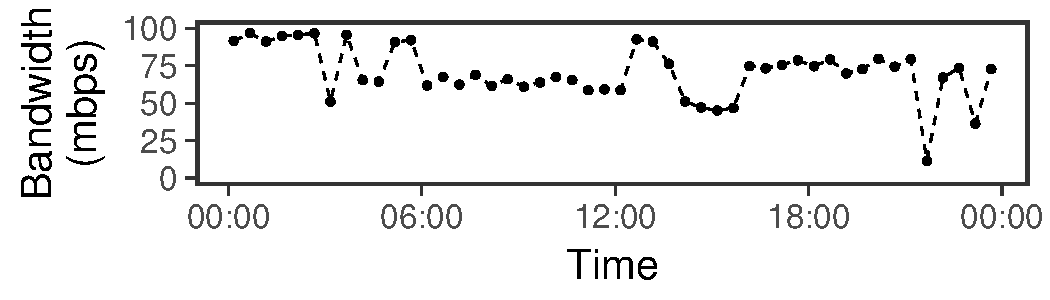
\includegraphics[width=.9\linewidth]{figures/aws-variation.pdf}
  \caption{Bandwidth variations throughout the day between Amazon EC2 sites
    (from Ireland to California).}
  \label{fig:bw}
\end{figure}

\begin{figure*}
  \centering
  \includegraphics[width=0.95\linewidth]{figures/motiv-app-specific.pdf}
  \caption{The measured bandwidth and application accuracy for two video analytics applications.
  (1) Different degradation strategies have different impacts on accuracy, e.g., degrading frame rate in (a) vs.\,degrading resolution in (b).
  (2) The same degradation strategy has different impacts on different applications, e.g., degrading frame rates works well for stationary camera (a), but not well for mobile camera (e). (c-g) shows example measurement frames.}
  \label{fig:app-specific}
\end{figure*}

\section{Motivation}
\label{sec:motivation}

In this section, we examine the gap between high application demands and limited
wide-area bandwidth. We then show that neither manual policies nor
application-specific optimizations solve the problem.

\subsection{Wide-area Streaming Applications}
\label{sec:wide-area-streaming}

\paraf{Video Surveillance.} We envisage a city-wide monitoring system that
aggregates camera feeds---from stationary ground cameras and moving aerial
vehicles---and analyzes video streams in real-time for surveillance, anomaly
detection or business intelligence~\cite{oh2011large}. Traditionally, video
analysis has relied on humans, but recent advances in computer vision and deep
learning have dramatically increased accuracy for automatic visual scene analysis,
such as pedestrian detection~\cite{dollar2012pedestrian}, vehicle
tracking~\cite{coifman1998real}, an facial recognition to locate people of
interest~\cite{parkhi2015deep, Lu:2015:SHF:2888116.2888245}. While some
surveillance networks use dedicated links, an increasing number of surveillance
systems, such as Dropcam~\cite{dropcam} and Vigil~\cite{zhang2015design}, use
the public Internet and wireless links to reduce the cost of deployment and
management.

% \para{High-frequency IoT Sensors:} Although environmental sensors used to be
% slow and not data-intensive~\cite{atzori2010internet}, increasingly,
% high-frequency, high-precision sensors are deployed. For example, uPMUs
% monitor the electrical grid with a network of 1000 devices; each produces 12
% streams of 120 Hz high-precision values accurate to 100 ns. This amounts to
% 1.4 million points per second~\cite{andersen2016btrdb}.

\para{Infrastructure Monitoring.} Large organizations today are managing
10--100s of data centers (DCs) and edge clusters
worldwide~\cite{calder2013mapping}. This geo-distributed infrastructure
continuously produces large volumes of data such as data access logs, server
monitoring logs, and performance counters~\cite{pu2015low,
  alspaugh2014analyzing, vulimiri2015global}. While most log analysis today runs
in batch mode on a daily basis, there is a trend towards analyzing logs in real
time for rapid optimization~\cite{rabkin2014aggregation}. For example, CDNs can
improve the overall efficiency by optimizing data placement if the access logs
can be processed in real time.

%% ~\cite{xu2009detecting} We generated the HDFS logs by setting up a Hadoop
%% cluster on 203 EC2 nodes and running sample Hadoop map-reduce jobs for 48
%% hours, generating and processing over 200 TB of random data. We collected
%% over 24 million lines of logs from HDFS.

% We consider the practical issues with deploying these applications in the
% wide-area. Our stand is that these applications face a bigger network
% challenge.  Data generated from the edge often fail to be delivered to the
% processing site because of the scarce and variable bandwidth capacity in the
% wide-area. Once they arrive, existing stream processing systems can easily
% manage a large cluster and perform data analytics at real-time.

\subsection{Wide-area Bandwidth Characteristics}
\label{sec:wide-area-bandwidth}

WAN bandwidth is insufficient and costly, as demonstrated by recent WAN-aware
systems~\cite{pu2015low, vulimiri2015global, vulimiri2015wananlytics,
  hsieh17gaia}. Using Amazon EC2 as a case study, the WAN bandwidth capacity is
15x smaller than their LAN bandwidth on average, and up to 60x smaller in the
worst case~\cite{hsieh17gaia}. In terms of pricing, as of April 2017, the
average WAN bandwidth cost is up to 38x of the cost of renting two
machines~\cite{amazon2017pricing, hsieh17gaia}.

In addition to the scarcity and cost, the large variability of WAN bandwidth
also affects streaming workloads. We conducted a day-long measurement using
iPerf~\cite{iperf3} to measure pair-wise bandwidth between four Amazon EC2
sites. The results show large variance in all pairs---\autoref{fig:bw} is one
such pair. There are occasions when available bandwidth is below 25\% of the
maximum bandwidth.

The back-haul links between EC2 sites are better---if not at least
representative---in comparison to general WAN links. Similar scarcity and
variations have been reported in wireless networks~\cite{biswas2015large},
broadband access networks~\cite{grover2013peeking, sundaresan2014bismark} and
cellular networks~\cite{nikravesh2014mobile}.

\subsection{The Case for a System Approach}
\label{sec:making-case-sys-approach}

To address the bandwidth limits, existing solutions include manual policies and
application-specific solutions. We discuss their drawbacks to make the case for
a system approach.

\para{Manual polices are sub-optimal.} While existing systems such as
JetStream~\cite{rabkin2014aggregation} and DASH~\cite{sodagar2011mpeg} allow
adaptation, they require developers to write manual policies. We illustrate the
problems with manual policies using an example~\cite{rabkin2014aggregation}:
\textit{if bandwidth is insufficient, switch to sending images at 75\% fidelity,
  then 50\% if there still isn't enough bandwidth. Beyond that point, reduce the
  frame rate, but keep the image fidelity.}

First, this policy is not accurate.
Developers write such rules based on heuristics and
don't back them up with measurements. Images with 75\% fidelity do not
necessarily lead to 75\% application accuracy. In terms of bandwidth, naively
one would think that reducing the frame rate by half will also half the data
rate. But if video encoding such as H.264~\cite{richardson2011h} is used, a reduction in frame rate increases the inter-frame difference, creating
larger P-frames. \hyperref[fig:app-specific]{Fig.~3e} shows that by reducing the
frame rate to one-third (from \(30~\text{FPS}\) to \(10~\text{FPS}\)), the bandwidth demand is still more than 50\%.

Second, it is not scalable to specify rules in this way. When the policy involves multiple dimensions
or developers desire a fine-grain control, the policy will end up with too many
rules.  Writing such rules manually is a tedious and error-prone process.

Lastly, this abstraction is too low-level. It forces developers to study and measure the
impact of individual operations, prohibiting its wide adoption in practice.

\para{Application-specific solutions don't generalize.} Because each application
has a different performance metric, relies on different features, and targets
different data distributions, a fine-tuned policy for one application will often work
poorly for others.

Analytical applications have their own goals, entailing different optimization metrics and
different algorithms.
%
%For instance, traditional video streaming focuses on end-users'
%experience~\cite{yin2015control, michalos2012dynamic, pantos2016http}. If we
%transfer their techniques to %machine-based video analytics, the %system maintains
%an unnecessarily-high frame rate.
%
In video analytics, for instance,
object detection algorithms depend on the edge
information~\cite{canny1986computational, lowe2004distinctive, viola2001rapid}
while object tracking~\cite{allen2004object} works best when the inter-frame
difference is small. The former is sensitive to resolution changes while the
latter frame rate changes.

Similar applications face different data distributions. Compare the stationary
camera detecting pedestrians with the mobile camera recognizing objects
(\autoref{fig:app-specific}). In the former case, when we take the pedestrians'
walking speed into consideration, a high frame rate is not necessary. But
high-resolution images are crucial as surveillance cameras are far from the
targets. In the latter case, mobile cameras move. Reducing the frame rate
introduces significant errors.

%%% Local Variables:
%%% mode: latex
%%% TeX-master: "awstream"
%%% End:

\section{System Overview}
\label{sec:system-overview}

\subsection{Developer APIs}
\label{sec:developer-apis}

We take inspiration from various stream processing framework proposed earlier
(such as JetStream, Apache Flink) and have designed our APIs. Although it's not
part of our main contribution, we include it for the completeness of our work
and to assist the discussion of adaptive APIs.

\subsection{System Architecture}
\label{sec:system-architecture}

System architecture: figure show each components

\subsection{Challenges}
\label{sec:challenges}

We outline the challenges, which will be extended in \autoref{sec:system-design}.

\begin{itemize}
\item Profiling
\item Per-task adaptation
\item Inter-task allocation
\item Processing placement
\end{itemize}

%%% Local Variables:
%%% mode: latex
%%% TeX-master: "sigcomm2017"
%%% End:

\section{System Design}
\label{sec:system-design}

In this section, we dive into each component of \sysname{}; we focus on
degradation and adaptation, rather than being verbose on every component.

Applications in \sysname{} are composed by connecting a set of operators to form
a dataflow processing graph. Our system provides basic set of APIs such as
\texttt{map}, \texttt{filter}, \texttt{window} (\autoref{tab:operators}). The
normal operators are similar to existing stream processing systems; our
contribution is the set of APIs to allow the specification of degradation
operations for bandwidth-accuracy trade-off.

\begin{table*}
  \centering
  \begin{tabular}{ c r l }
    \toprule
    \multirow{7}{*}{Normal Operators}
    & \textit{map}(f: I $\Rightarrow$ O) & Stream<I> $\Rightarrow$ Stream<O> \\
    & \textit{filter}(f: I $\Rightarrow$ bool) & Stream<I> $\Rightarrow$
                                                 Stream<I> \\
    & \textit{skip}(i: Integer) & Stream<I> $\Rightarrow$ Stream<I> \\
    & \textit{sliding\_window}(count: Integer, f: Vec<I> $\Rightarrow$ O) & Stream<I> $\Rightarrow$
                                                                            Stream<O> \\
    & \textit{tumbling\_window}(count: Integer, f: Vec<I> $\Rightarrow$ O) & Stream<I> $\Rightarrow$
                                                                             Stream<O> \\
    & \textit{timed\_window}(time: Duration, f: Vec<I> $\Rightarrow$ O) & Stream<I> $\Rightarrow$
                                                                          Stream<O> \\
    & ... & ... \\
    \midrule
    \multirow{4}{*}{Degradation Operators}
    & \textit{maybe}(knobs: Vec<T>, f: (T, I) $\Rightarrow$ I) & Stream<I> $\Rightarrow$
                                                                 Stream<I> \\
    & \textit{maybe\_skip}(knobs: Vec<T>) & Stream<I> $\Rightarrow$ Stream<I> \\
    & \textit{maybe\_downsample}(knobs: Vec<(Integer, Interger)>) & Stream<Image> $\Rightarrow$ Stream<Image> \\
    & ... & ... \\
    \bottomrule
  \end{tabular}
  \caption{A comparison between normal stream processing operators and our
    degradation operators. Vec<T> represents a list of elements of type
    T. Option<T> indicates an element of type T can be absent. Notice the type
    constrain on the \texttt{maybe} function while \texttt{maybe\_map} relaxes
    it.}
  \label{tab:operators}
\end{table*}

\subsection{Degradation Operators}
\label{sec:prog-abs}

We first consider a strawman solution: manual policies for
degradation. JetStream~\cite{rabkin2014aggregation} offers an example: ``if
bandwidth is insufficient, switch to sending images at 75\% fidelity, then 50\%
if there still isn't enough bandwidth. Beyond that point, reduce the frame rate,
but keep the images at 50\% fidelity.'' We identify the following issues with
this approach.

\para{Lack of precision:} These policies are often developer heuristics and
rarely backed up by measurements. First, there is no direct association of the
application accuracy with the 75\% fidelity configuration. Besides, their impact
on the data size is also not trivial.  While it seems intuitive that the level
of degradation will affect the data size, the precise impact is not always
straightforward. For example, one might think that reducing the frame rate by
50\% will half the data rate. When video encoding is employed, the inter-frame
difference will increased (P-frame size) when the frame rate is reduced. This
leads to a larger data size for each frame. \autoref{fig:h264} illustrates this
complex relationship with an example of H.264 encoding under four different
frame rates.

\para{Not scalable:} The strawman solution quickly leads to too many policies
when multiple degradation operations are involved or a fine-grained control is
desired. This manual process becomes tedious and error-prone. When too few rules
are provided, the application may oscillate between two rules: one that's too
aggressive (always faces insufficient bandwidth) and one that's too
conservative.

\begin{figure}
  \centering
  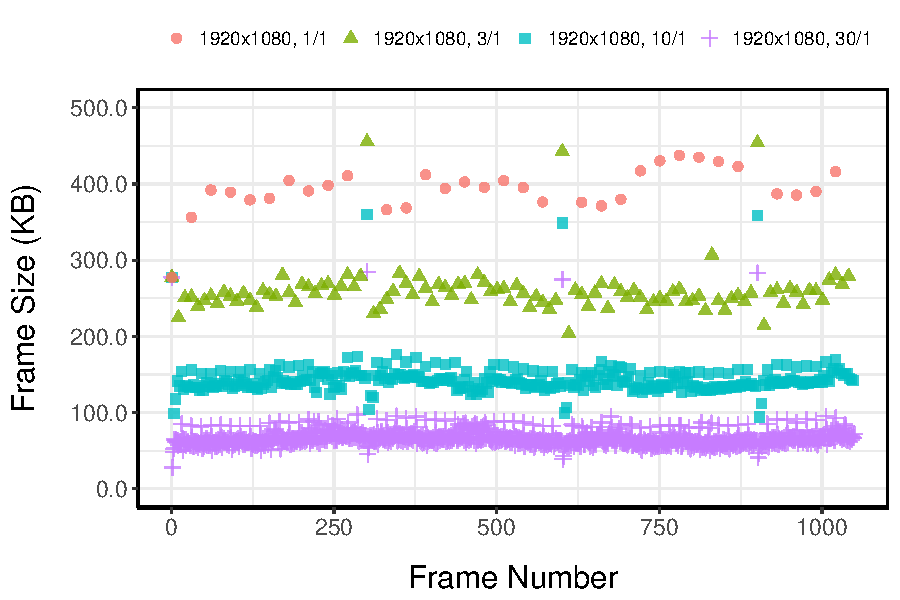
\includegraphics[width=\columnwidth]{figures/h264.pdf}
  \caption{H.264 requires more information per frame when the frame rate is
    reduced.}
  \label{fig:h264}
\end{figure}

\vspace{0.5em}

When using the above strawman solution, developers are forced to manually study
and measure the impact of individual degradation policy, prohibiting its wide
adoption in practice.

On the other extreme of the design spectrum, a completely developer-free
solution is not practical. While static analysis has been shown to optimize
application execution adaptively in a certain context~\cite{chun2011clonecloud},
they do not work well in our dataflow programming model. Static analysis is
prone to false positives: exploring wrong or unnecessary parameters. For
example, when the application is configured to generates statistics with a
\texttt{timed\_window} operation, static analysis may falsely detect the
duration parameter and alter the behavior of the application in an unexpected
way. Also, as we will illustrate in~\autoref{sec:profiling}, with each
introduced parameter, the profiling time increases drastically as all parameters
pose a combinatorial space.

Our system take a middle ground between these two extremes: developers use a
novel \texttt{maybe} API to annotate degradation operations without being exact
on the values. Think of these APIs as hints from developers: this operation,
when in use, will likely reduce the data size and affect the data fidelity;
however the exact impact is not clear.

The basic form of \texttt{maybe} operator takes two arguments: a knob and a
degradation function (see \autoref{tab:operators}). The knob indicates different
degradation levels; the function performs the actual degradation operation with
a configurable level. We restrict the type signature of the function that this
API can accept: $f(T, I) \Rightarrow I$. That is, the degradation function
should not alter the type of the stream. While this might seem a strong
restriction, when combined with \texttt{map} operator, the system is still
expressive enough. We describe our implementation and usage
in~\autoref{sec:implementation}.

\begin{sloppypar}
  Based on the \texttt{maybe} primitive, one can implement wrappers for common
  degradation operations. For example, \texttt{maybe\_skip} will optionally
  subsample a stream; and \texttt{maybe\_downsample} can adjust the image
  resolution to a configured target. With this API, the example mentioned
  earlier can now be implemented as follows:
\end{sloppypar}

\begin{lstlisting}
   let app = Camera::new((1920, 1080, 30))
      .maybe_downsample(vec![(1600, 900), (1280, 720)])
      .maybe_skip(vec![2, 5])
      .map(|frame| frame.show())
      .compose();
\end{lstlisting}

This snippet first instantiate a \texttt{Camera} source, which is a
\texttt{Stream<Image>} with 1920x1080 resolution and 30 FPS. Two degradation
operations are chained after the source: one that downsample the resolution to
either 1600x900 or 1280x720; the other skip the frame with a parameter of 2 or
5, resulting in 30/(2+1)=10 FPS or 30/(5+1)= 6 FPS. After the degradation,
images are shown on the display. In practice, further processing operators can
be chained.

While the API itself has simplified the specification of degradation, the exact
amount has to be known for precise rate adjustment at runtime. We then turn to
the second stage of our system that performs automatic profiling.

%%% Local Variables:
%%% mode: latex
%%% TeX-master: "sigcomm2017"
%%% End:

\section{Implementation}
\label{sec:implementation}

In this section we present details about our implementation, including a
prototype framework and three non-trivial wide-area streaming applications.
\sysname{} is implemented in Rust and open-source on Github.\footnote{Url elided
  for anonymity.}

\subsection{Framework}
\label{sec:framework}

While our proposed APIs are general enough that they can be implemented in most
languages, we chose a safe language, Rust, to implement the core framework for
the following reasons. First, Rust's memory safety guarantee can ensure
applications running continously for an extended period of time. Besides, the
zero-cost abstraction removes the possibilities of tail latencies caused by
uncoordinated garbage collection~\cite{maas2016taurus}. In addition, we rely on
Rust's type system to enforce the type match on \texttt{maybe} operations.

Our basic APIs are similar to existing stream processing
frameworks. Applications are modelled as a graph of computations where basic
operators such as \texttt{window}, \texttt{map}, \texttt{filter} are provided.
For brevity, we do not dive into details of these operators. Instead, we focus
the discussion on our degradation operations.

All operators implement the \texttt{Stream} trait which has an associate type
\texttt{Item} and a core function \texttt{next} that returns \texttt{Datum}:
it's either an item or an error. The concrete form of \texttt{maybe} API is as
follows.

\begin{lstlisting}
pub trait Stream {
    type Item;
    fn next(&mut self) -> Datum<Self::Item, Error>;

    fn maybe<K, F>(self, opts: K, f: F) -> Maybe<Self, F>
        where Self: Sized,
                K: IntoKnob,
                F: FnMut(K::Item, Self::Item) -> Self::Item {

         // omitted
    }
}

pub trait IntoKnob {
    fn into_knob(self) -> Knob;
}
\end{lstlisting}

Developers can directly use the above API with user-defined functions, such as
the following example.

\begin{lstlisting}
let quantized_stream = vec![1, 2, 3, 4, 5, 6]
    .into_stream()
    .maybe(vec![2, 3], |knob, p| p % knob);
    .collect();
\end{lstlisting}

Alternatively, the API can be extended to support common operators. For example,
\texttt{maybe\_downsample} operator can that uses the \texttt{downsample}
function internally. This function takes two argument: target size specified
using a tuple and the image.

\begin{lstlisting}
fn downsample(res: (usize, usize), image: Mat) -> Mat {

    //  omitted

}
\end{lstlisting}

Our current prototype is about 2000 lines of code, with heavy use of open-source
libraries.

Applications built with \sysname{} runs as a single process. The entire
processing pipeline is often specified in a single main file. The execution mode
(profiling, runtime as client or runtime as server) is configured with command
line arguments or environment variables (similar to how
\texttt{nc}/\texttt{iperf} works). The deployment manager is using Docker
container for the deployment task.

\subsection{Building \sysname{} Applications}
\label{sec:build-appl}

We built three applications (\autoref{fig:apps}) using \sysname{}: pedestrian
detection surveillance, an augmented reality and distributed Top-K. We focus on
the application-specific part---knobs, utility function and
dataset. \autoref{tab:apps} summarizes the 

\begin{table*}
  \centering
  \begin{tabular}{|c|c|c|c|}
    \hline
    Application & Knobs & Utility & Dataset \\
    \hline
    Pedestrian Detection & resolution, framerate, quantizer
                        & F1 score & MOT16-04 (training), MOT16-03 (testing) \\
    \hline
    Augmented Reality & resolution, framerate, quantizer
                        & F1 score & Video clips of office (training), home (testing) \\
    \hline
    Top-K & head (N), local threshold (T) & Kendall's W & sec.gov access log
                                                          (4 days training, 12 days testing)  \\
    \hline
  \end{tabular}
  \caption{\sysname{} Applications}
  \label{tab:apps}
\end{table*}

\begin{figure*}
  \centering
  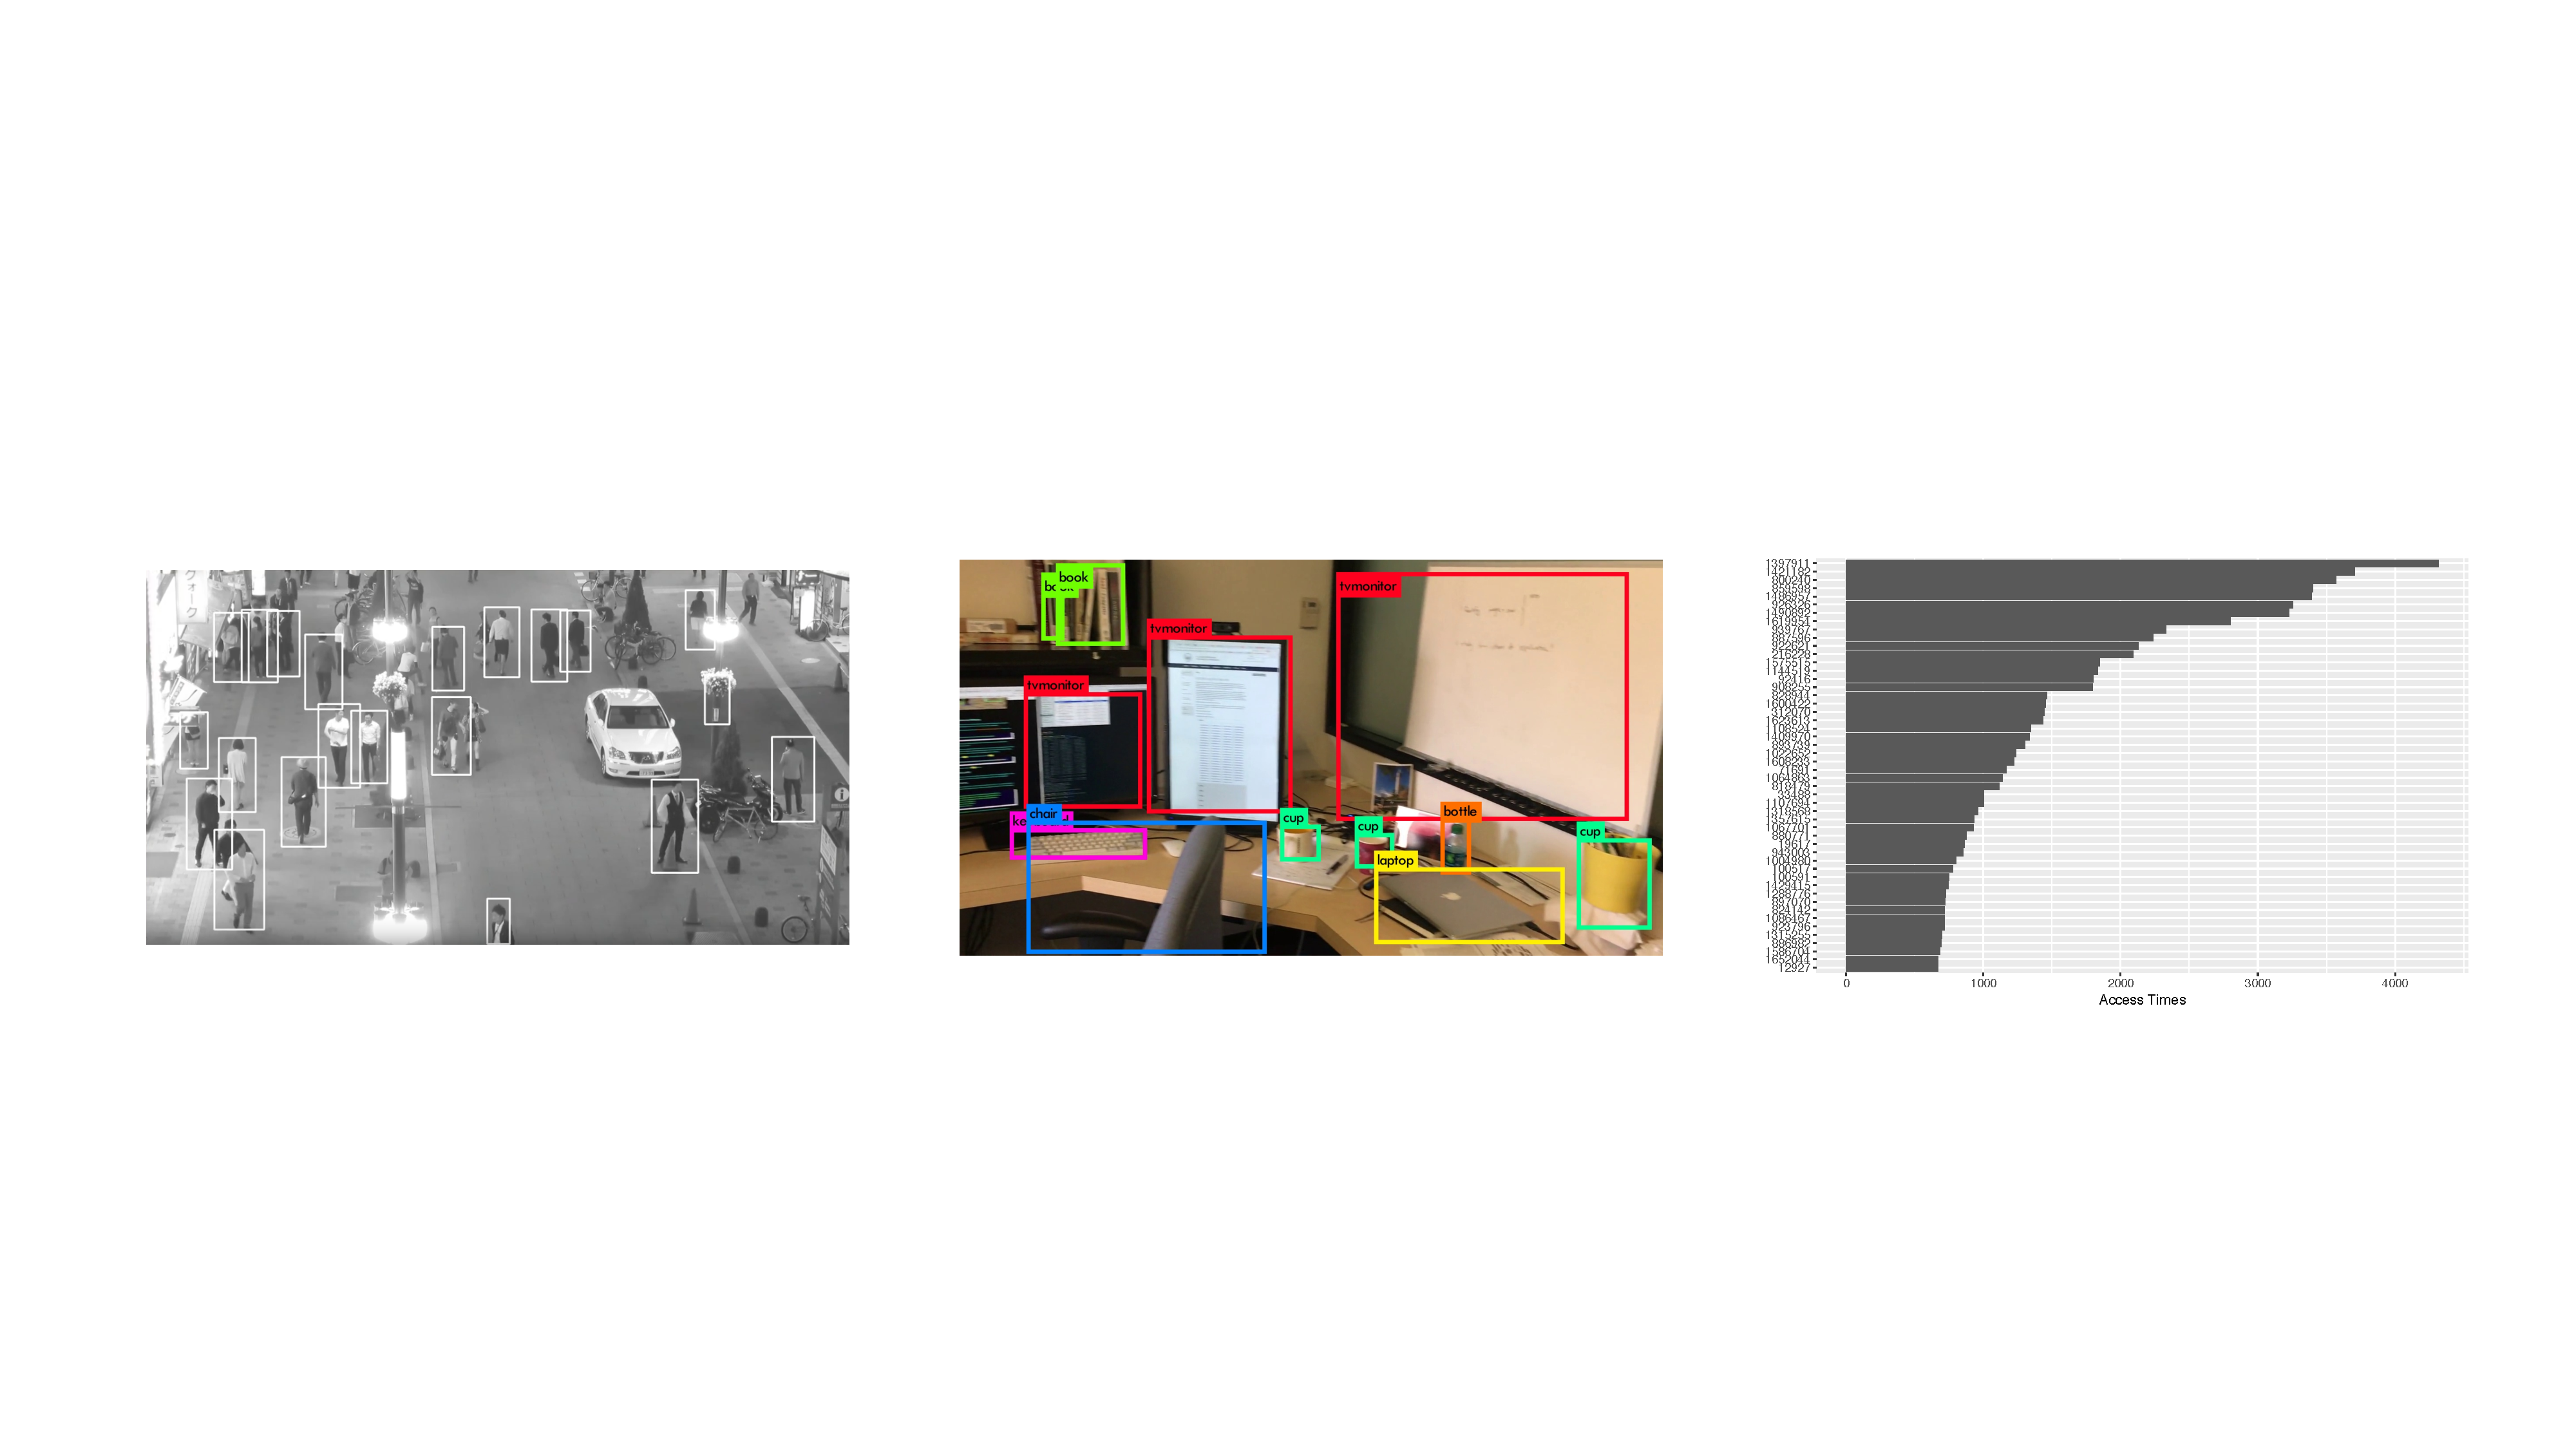
\includegraphics[width=.95\textwidth]{figures/apps.pdf}
  \caption{\sysname{} applications}
  \label{fig:apps}
\end{figure*}

\para{Pedestrian Detection:} This application analyzes video streams from
installed CCTV cameras and detect pedestrians inside. The detection result is a
list of bounding boxes representing pedestrian's relative location within the
view. Variant of this application can be used for safety monitoring, anomaly
detection or waiting line counting.

We implement most image-related operations using OpenCV
3.1~\cite{opencvlibrary}. The pedestrian detection uses histogram of oriented
gradients (HOG)~\cite{dalal2005histograms} with the default linear SVM
classifier. To ensure real-time processing of frames, GPU-accelerated
implementation is used in favor of the CPU-based implementation.

For video encoding, H.264 scheme is chosen for its prevalence in existing
systems. Our implemenation is based on GStreamer~\cite{gstreamer}, using
\texttt{x264enc} plugin. To integrate with \sysname{}, we create a pipeline that
exposes \texttt{appsrc} (to feed raw image data) and \texttt{appsink} (to get
encoded bytes). The GStreamer main loop is managed in a separate thread and
\sysname{} communicate with it via Rust's channel. The \texttt{x264enc} is
configured with \texttt{zerolatency} present and runs using four threads. It
uses constant quality encoding and the quantizer is exported as a parameter that
can be tuned.

This application has three degradation operations: reducing image resolution,
dropping frame rate or lower video encoding quality. We use F1 score as the
utility function. F1 score (\%) is the harmonic mean of precision and
recall~\cite{Rijsbergen:1979:IR:539927}. Here a successful detection is defined
when the intersection over union (IOU) is greater than
50\%~\cite{everingham2010pascal}.

\para{Augmented Reality:} We target at mobile augmented reality applications
which offload the heavy computation to resources elsewhere. Although local
computation is gaining attraction~\cite{satyanarayanan2009case, zhang2015cloud},
wireless communication link is also susceptible to capacity variation.

We use a similar setup as the pedestrian detection application except the actual
function that analyzes the stream. To recognize objects, we use a a pre-trained
neural network~\cite{darknet13} that's trained with
Imagenet~\cite{krizhevsky2012imagenet}. Similar to our first application,
GPU-accelerated implementation is use in favor for real-time processing.

The utility function here is more strict than the pedestrian detection:
true-positive depends not only on IOU criteria, but also on the type of objects
(a correct identification).

\para{Distributed Top-K:} Many distributed system monitoring applications
require to answer the ``top-k'' question~\cite{babcock2003distributed}, such as
the top-k most popular URLs or the top-k most access files. Naive methods of
transmitting all the raw log entries to the aggregation point is not feasible as
popular servers typically have millions of requests per second. Local worker
node can first perform a transformation that generates data summary, such as
key-value pairs of \texttt{<item, count>}. Even after this operation, the data
size could still be large given most real-world access patterns follow a
long-tailed distribution. There is a large-but-irrelevant tail that may be
unnecessary to send.

We consider two degradation operations: (1) a \texttt{head} operation that
performs a local Top-\texttt{N} first; (2) a local threshold \texttt{T} that
filters the tail. Obviously, these two operations are not orthognal to each
other. The impact on data size and quality depends on the distribution of the
actual data.

To evaluate the degradation impact, we use Kendall's W, which is a distance
measure of the concordance between two ranked list. The function outputs a
statistic measure ranging from 0 to 1, representing no agreement to complete
aggrement, respectively~\cite{abdi2007kendall}.

%%% Local Variables:
%%% mode: latex
%%% TeX-master: "sigcomm2017"
%%% End:

\begin{figure*}[htb]
  \centering
  \begin{subfigure}[t]{0.32\textwidth}
    \centering
    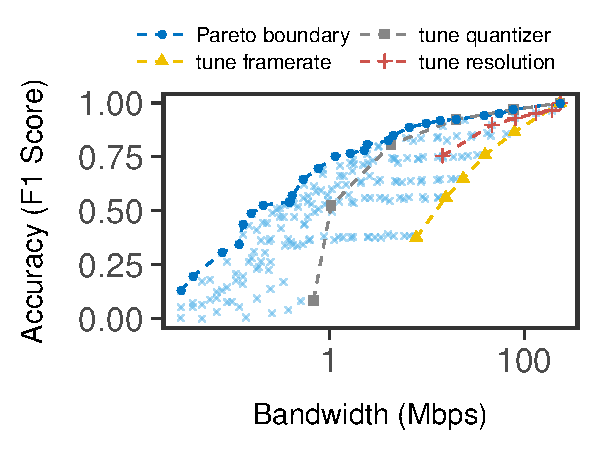
\includegraphics[width=\textwidth]{figures/profile-darknet.pdf}
    \caption{Augmented Reality (AR)}
    \label{fig:ar-profile}
  \end{subfigure}
  \hfill
  \begin{subfigure}[t]{0.32\textwidth}
    \centering
    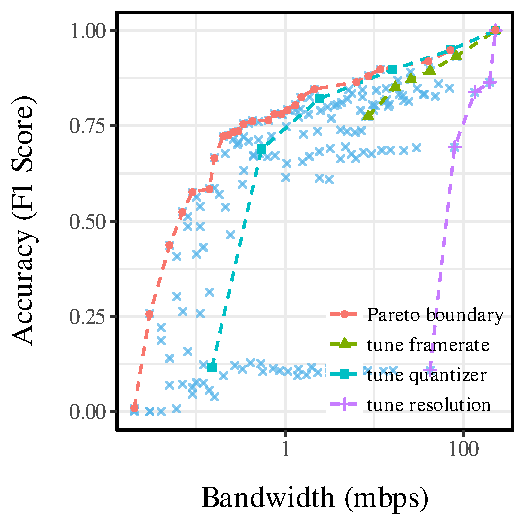
\includegraphics[width=\textwidth]{figures/profile-mot.pdf}
    \caption{Pedestrian Detection (PD)}
    \label{fig:pd-profile}
  \end{subfigure}
  \hfill
  \begin{subfigure}[t]{0.32\textwidth}
    \centering
    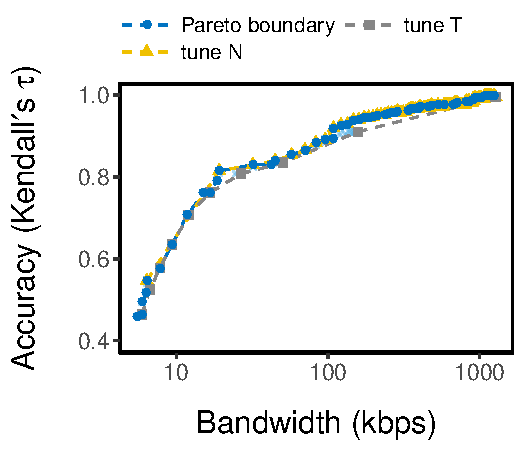
\includegraphics[width=\textwidth]{figures/profile-topk.pdf}
    \caption{Top-K (TK)}
    \label{fig:tk-profile}
  \end{subfigure}
  \caption{Application profiles of three applications. Each cross point is one
    configuration $c$'s performance $(B(c), A(c))$. All figures show the Pareto
    boundary as well as the performance if only tuning one dimension. Note the
    x-axis is in log scale.}
  \label{fig:all-profiles}
  \vspace{-0.5em}
\end{figure*}

\section{Evaluation}
\label{sec:evaluation}

In this section, we show the evaluations of \sysname{}, summarizing the results
as follows.

\begin{itemize}[itemsep=0pt, topsep=3pt]
\item[\autoref{sec:application-profiles}] \sysname{} generates Pareto-optimal
  profiles across multiple dimensions with precision
  (\autoref{fig:all-profiles}).
\item[\autoref{sec:online-profiling}] Our parallel and sampling techniques
  speeds up offline and online profiling (\autoref{fig:parallel},
  \autoref{fig:online-tricks}).
\item[\autoref{sec:runtime-adaptation}] At runtime, all \sysname{} applications
  achieve sub-second latency and nominal accuracy drop
  (\autoref{fig:ar-runtime}, \autoref{fig:pd-runtime},
  \autoref{fig:tk-runtime}).
\item[\autoref{sec:various-rtt}] \sysname{} maintains low latency performance
  across different network conditions (\autoref{fig:ar-rtt}).
\item[\autoref{sec:multi-task-alloc}] \sysname{} profiles allow different
  resource allocations: resource fairness and utility fairness
  (\autoref{fig:multitask}).
\end{itemize}

\subsection{Application Profiles}
\label{sec:application-profiles}

We run offline profiling using the training dataset described
in~\autoref{tab:apps} and show the learned profiles in
\autoref{fig:all-profiles}. In each figure, the cross dots represent the
bandwidth demand and application accuracy for one configuration. We highlight
the Pareto-optimal boundary $\mathbb{P}$ with blue dashed lines. To understand
each dimension's impact on the degradation, we highlight configurations from
tuning only \textit{one} dimension. From these profiles, we make the following
observations:

\para{Large bandwidth variation.} For all three applications, The bandwidth
requirements of all three applications have two to three orders of magnitude of
difference (note the x-axis is in log scale). For AR and PD, the most expensive
configuration transmits videos at 1920x1080, 30 FPS and 0 quantization; it
consumes \SI{230}{Mbps}. In contrast to the large bandwidth variation, there is
a smaller variation in accuracy. In PD, for example, even after the bandwidth
reduces to \SI{1}{Mbps} (less than 1\% of the maximum), the accuracy is still
above 75\%. The large variation allows \sysname{} to operate at a high accuracy
configuration even under severe network deterioration.

\para{Distinct effects by each dimension.} Comparing dashed lines in each
profile, we see that the Pareto-optimal configurations are only achievable when
multiple knobs are in effect. Tuning only one dimension often leads to
sub-optimal performance. Within a single profile, the difference between tuning
individual dimensions is evident. For PD, tuning resolution (the red line) leads
to a quicker accuracy drop than tuning frame rate (the yellow line). Comparing
AR and PD, the same dimension has different impact. Tuning resolution is less
harmful in AR than PD; while tuning frame rate hurts AR more than PD\@. This
echoes our initial observation in~\autoref{subsec:motivation} that
application-specific optimizations do not generalize.

% \para{Quantification with precision}. The generated profiles are actionable
% configurations that control the knobs with precision. For example, if PD
% transmits video at 1920x1080 resolution, \(10~\text{FPS}\) and a quantization
% of 20, it will consume 11.7 mbps of bandwidth, achieving roughly 90\%
% accuracy. This saves developers from laboriously analyzing their application
% to compute manual policies.

\subsection{Profiling Efficiency \& Online Profiling}
\label{sec:online-profiling}

This section focuses on the AR application as a case study; our profiling
techniques---parallelism and sampling---do not make assumptions about the
application; therefore, the evaluation results can be generalized to other
applications.

In AR, there are 216 different configurations: 6 resolutions, 6 frame rates and
6 quantization levels. AR uses YOLO~\cite{redmon2016yolo9000}, a neural network
model for object detection. It takes roughly \SI{30}{\ms} to process one frame
on GeForce\textregistered\space GTX 970.\footnote{YOLO resizes an input image to
  a fixed resolution (416x416) as required by the neural network. It takes a
  similar amount of time to Evaluating each image (with different resolutions).}
But different configurations require different times for processing. For
example, a \(10~\text{FPS}\) video has 1/3 of the frames to process in
comparison to a \(30~\text{FPS}\) video.  In our experiment, to evaluate all 216
configurations, it takes 52 seconds for 1 second worth of data. We denote such
overhead as 52X\@. \hyperref[sec:automatic-profiling]{Section 3.2} have
discussed parallel and sampling techniques to improve the profiling efficiency;
we present their evaluations as follows.

\begin{figure}
  \centering
  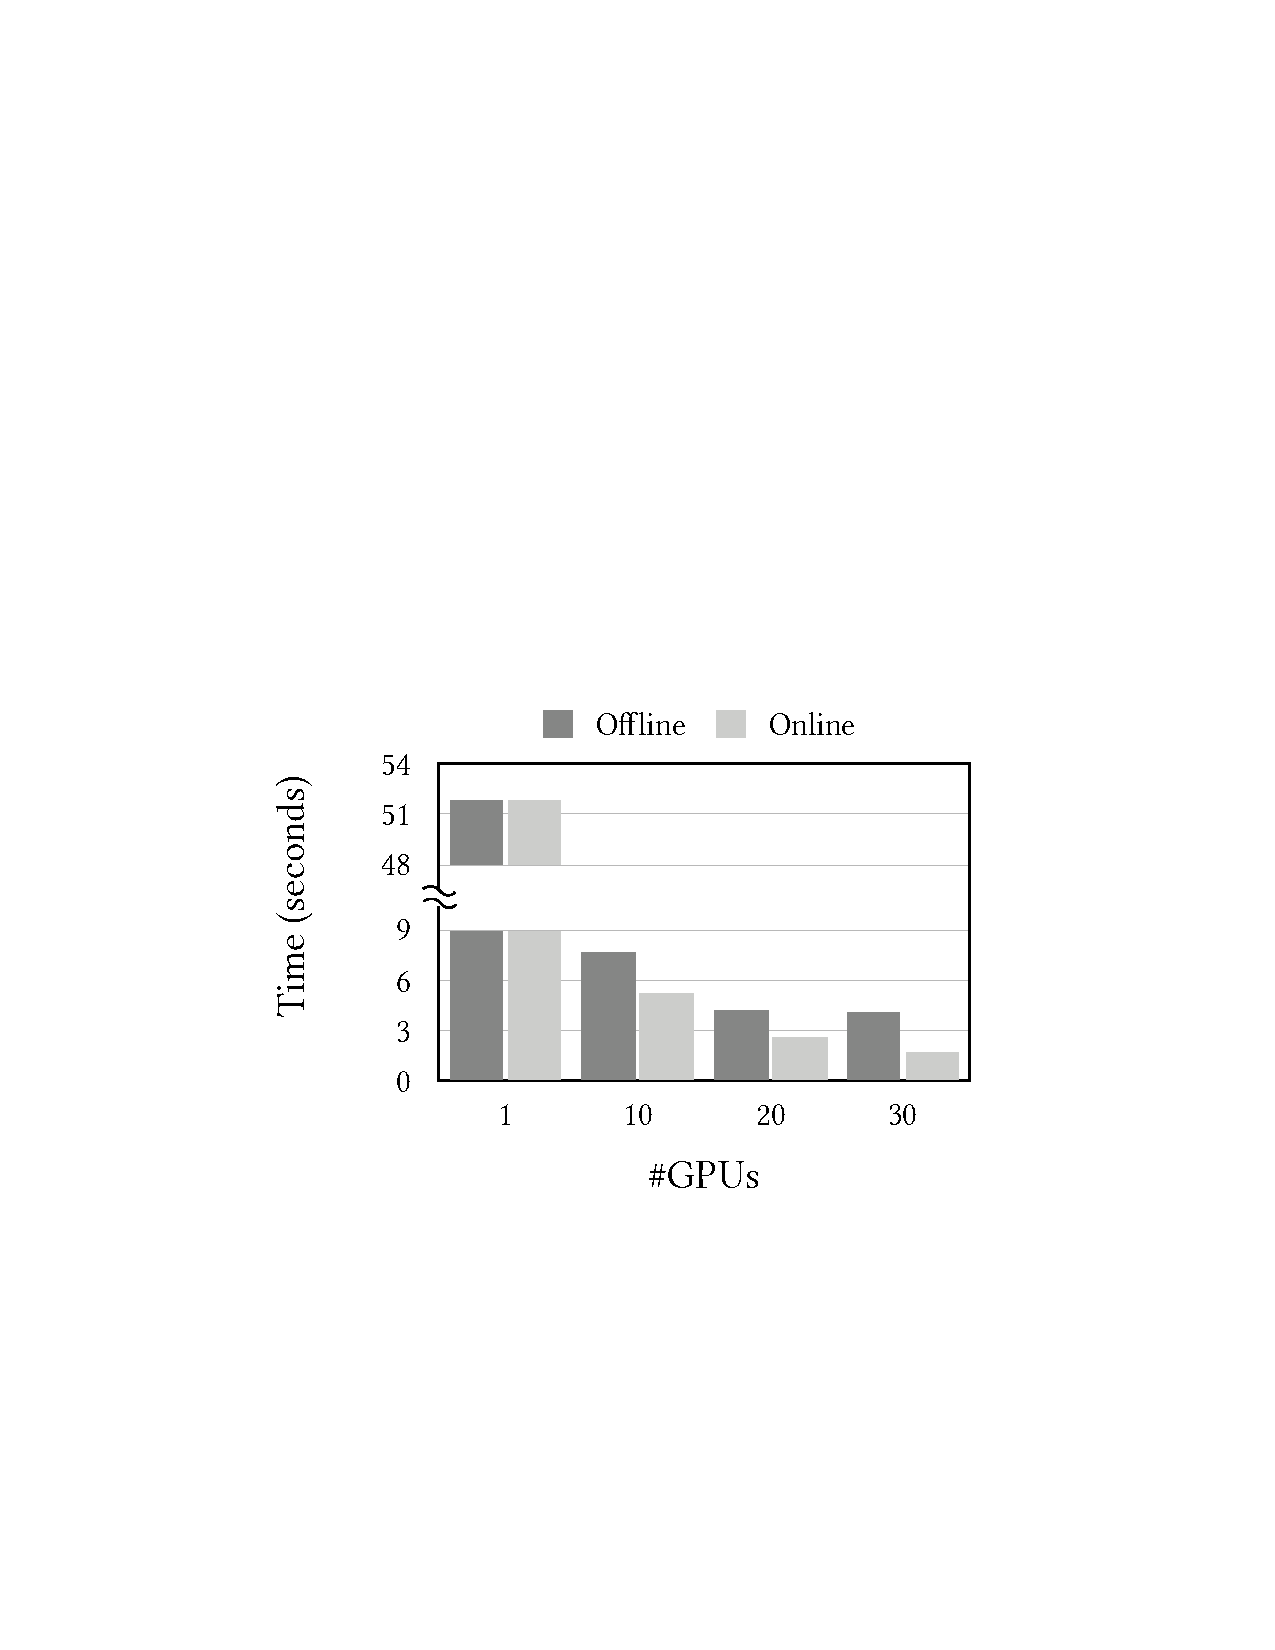
\includegraphics[width=1.0\columnwidth]{figures/parallel.pdf}
  \caption{Parallelism speeds up both offline and online profiling.
  The y-axis shows the profiling time for 1-second video.}
  \label{fig:parallel}
  \vspace{-0.5em}
\end{figure}

\para{Parallelism reduces the profiling time (\autoref{fig:parallel})}. Because
evaluating each individual configuration is independent of other configurations,
we parallelize the profiling task by assigning configurations to GPUs.
$(i)$~Our offline profiling assigns configurations randomly.  With the increased
number of GPUs, the overhead reduces from 52X to 4X with 30 GPUs.  $(ii)$~Our
online profiling assigns configurations based on the processing times collected
during offline.  \sysname{} uses LFS~\cite{karger2010scheduling} to minimize the
makespan and reduces the overhead to 1.75X with 30 GPUs (29$\times$ gain).

\para{Sampling techniques speed up online profiling
  (\autoref{fig:online-tricks}).}  Before we evaluate the speed up, we validate
\textit{model drift} with real-world data. We use the profile trained in an
office environment.  According to the profile, the application should operate at
a configuration of 1280x720, \SI{30}{FPS} and 20 quantization to meet an
\SI{11}{Mbps} goal.  We test it against a home environment, and at about t=100s,
the camera points out of the window to detect objects on the street. Because of
the scene change, the configuration fails to predict runtime bandwidth, as
illustrated in \autoref{fig:offline}.

To correct the profile, if we continuously run the profiling online and update
the profile, the application will choose the right configuration to meet the
bandwidth limit.  \autoref{fig:online} shows the bandwidth prediction when we
continuously profile with the past 30 seconds of video. At time t=120s, the new
prediction corrects the drift. The downside of continuous profiling, as
discussed earlier, is the cost: 52X overhead with 1 GPU\@. In addition to
parallelism, \sysname{} uses sampling techniques for online profiling
(improvements in \autoref{tab:online}):

(i) Partial data. Instead of using all the past data, we run profiling with only
a fraction of the raw data.  \autoref{fig:online-partial} shows the bandwidth
consumption if the profiling uses only 10 seconds of data out of the past 30
seconds. In this way, although the profile may be less accurate (the
mis-prediction at t=80-100s), and there is a delay in reacting to data change
(the mis-prediction is corrected after t=125s), we save the online profiling by
3$\times$ (from 52X to 17X).

(ii) Partial configurations. If we use the past profile as a reference and only
measure a subset of all Pareto-optimal configurations, the savings can be
substantial. A full profiling is only triggered if there is a significant
difference. \autoref{fig:online-trigger} shows the bandwidth prediction if we
evaluate 5 configurations continuously and trigger a full profiling when the
bandwidth estimation is off by \SI{1}{Mbps} or the accuracy is off by 10\%.  For
our test data, this scheme is enough to correct model drifts by predicting an
accurate bandwidth usage (compare \autoref{fig:online} and
\autoref{fig:online-trigger}).  The overhead reduces to 6X because we run full
profiling less often (only two full profiling). It is an 8.7$\times$ gain.

\begin{figure}
  \centering
  \begin{subfigure}[t]{0.45\columnwidth}
    \centering
    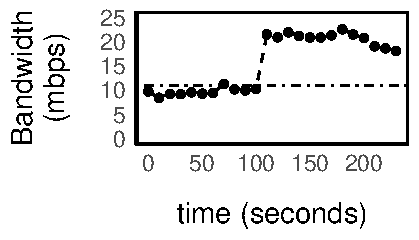
\includegraphics[width=\textwidth]{figures/online1.pdf}
    \caption{Offline only}
    \label{fig:offline}
  \end{subfigure}
  \hfill
  \begin{subfigure}[t]{0.45\columnwidth}
    \centering
    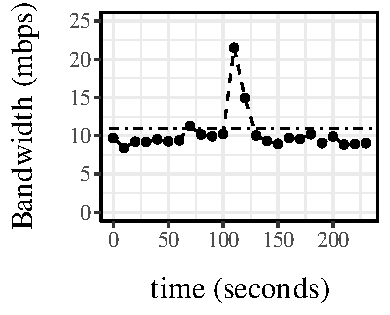
\includegraphics[width=\textwidth]{figures/online2.pdf}
    \caption{Online (continuous)}
    \label{fig:online}
  \end{subfigure}
  \\
  \vspace{0.5em}
  \begin{subfigure}[t]{0.45\columnwidth}
    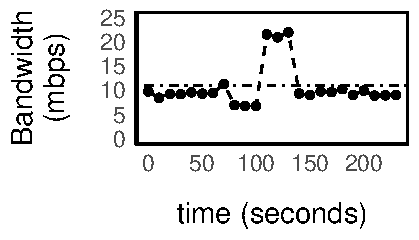
\includegraphics[width=\textwidth]{figures/online3.pdf}
    \caption{Partial data}
    \label{fig:online-partial}
  \end{subfigure}
  \hfill
  \begin{subfigure}[t]{0.45\columnwidth}
    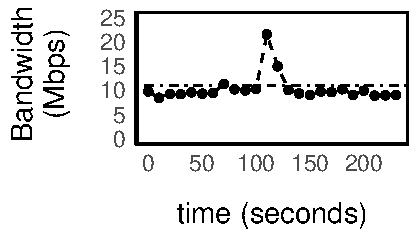
\includegraphics[width=\textwidth]{figures/online4.pdf}
    \caption{Partial configurations}
    \label{fig:online-trigger}
  \end{subfigure}
  \caption{The horizontal reference line is the target bandwidth
    (\SI{11}{Mbps}). (1) Online profiling is necessary to handle model drift
    ((a) vs.\,(b-d)). (2) Sampling techniques---partial data (c) and partial
    configurations (d)---can correct model drift with less profiling overhead
    (see \autoref{tab:online}), compared to continuous (b).  We omit accuracy
    predictions since in all schemes \sysname{} finds configurations that
    achieve similarly high accuracy (\textasciitilde 90\%).  }
  \label{fig:online-tricks}
  \vspace{-0.5em}
\end{figure}

%% Offline: 0
%% Online: 1 frame (1852.21 GPU * seconds)
%% Online (1/10)   (185.2 GPU * seconds)
%% Trigger         ( GPU * seconds)

\begin{table}[t]
  \small
  \centering
  \begin{tabular}{c c c}
    \toprule
    Online scheme & Overhead & Improvements \\
    \midrule
    Continuous & 52X & Baseline \\
    Partial data & 17X & 3$\times$\\
    Partial configurations & 6X & 8.7$\times$ \\
    \bottomrule
  \end{tabular}
  \caption{Compared to the continuous profiling baseline (52X overhead), our
    sampling techniques speed up by 3$\times$ or 8.7$\times$.}
  \label{tab:online}
  \vspace{-1em}
\end{table}

Note that these techniques---parallelization, sampling data, and sampling
configurations---can be combined together to further reduce the profiling
overhead. For example, scheduling five GPUs running 5 configurations
continuously to check for model drift will reduce the overhead to 1X\@. In
practice, the amount of resources to use depends on the budget and the
importance of the job. \sysname{} currently requires developers to configure the
application with proper online profiling techniques.

%% Note that it is not always needed to do online profiling. PD's test data
%% doesn't exhibit model drift.  Nor is online profiling always
%% expensive. Processing TK over all configurations.

\subsection{Runtime Adaptation}
\label{sec:runtime-adaptation}

In this section, we evaluate the runtime performance by controlling available
bandwidth across geo-distributed sites and compare \sysname{} with baselines
including streaming over TCP/UDP, JetStream, and video streaming. Our evaluation
shows that \sysname{} achieves low latency and high accuracy simultaneously
across all applications. We first discuss AR in depth and then present the
results of PD/TK.

\para{Experiment setup.} We conduct our experiments on four geo-distributed
machines from Amazon EC2, spanning four different regions. Three (at
N.\,Virginia, Ohio, Oregon) act as worker nodes and one (at N.\,California) acts
as the analytics server. The average RTTs from the workers to the server are
\SI{65.2}{\ms}, \SI{22.2}{\ms}, and \SI{50.3}{ms}.

During the experiment, each worker transmits test data (\autoref{tab:apps}) for
about 10 mins. If the duration of the test data is less than 10 mins, it
loops. Because $B(c_{\max})$ is prohibitively large (raw videos consumes
\SI{230}{Mbps} ), we use a reasonable configuration to limit the maximum
rate. In our AR experiment, $c_{\max}$ is 1600x900 resolution, \(30~\text{FPS}\)
and a quantization of 20; it consumes about \SI{14}{Mbps}.

Our bandwidth control scheme follows
JetStream~\cite{rabkin2014aggregation}. During the experiment, we use the Linux
\texttt{tc} utility with HTB~\cite{htb, lartc} to control the clients' outgoing
bandwidth. Each experiment involves four phases: $(i)$~before t=200s, there is
no shaping; $(ii)$~at t=200s, we limit the bandwidth to \SI{7.5}{Mbps} for 3
minutes; $(iii)$~at t=380s, we further decrease the available bandwidth to
\SI{5}{Mbps}; $(iv)$~ at t=440s, we remove all traffic shaping. For UDP, HTB
doesn't emulate the packet loss or out-of-order delivery; so we use
\texttt{netem} and configure the loss probability according to the delivery
rate. Because each pair-wise connection has a different capacity, we impose a
\textit{background} bandwidth limit---\SI{25}{Mbps}---to simplify comparisons.

We compare \sysname{} with the following baselines:

\begin{itemize}[noitemsep, nolistsep, leftmargin=*]

\item Streaming over TCP/UDP (non-adaptive). $(i)$~For TCP, we re-use
  \sysname{}'s runtime that runs over TCP but disable the adaptation. $(ii)$~For
  UDP, we use FFmpeg~\cite{bellard2012ffmpeg} to stream video:
  RTP/UDP~\cite{schulzrinne2006rtp} for media and RTSP for
  signaling~\cite{schulzrinne1998rtsp}. This is a common setup for video
  conferencing and IP cameras~\cite{durresi2005rtp, king2009cisco}.

\item Adaptive video streaming. We use HTTP Live Streaming (HLS) to represent
  popular adaptive video streaming techniques. Our setup resembles personalized
  live streaming systems~\cite{wang2016anatomy} but uses a smaller chunk for low
  latency (1 second instead of typical 2-10 seconds).\footnote{The appendix
    includes details about our HLS setup.}

\item JetStream with the manual policy described in \autoref{subsec:motivation}.

\item JetStream++, a modified version of JetStream that uses the profile learned
  by \sysname{}.\footnote{The appendix includes details about how we modified
    JetStream.}

\end{itemize}

At runtime, \sysname{} differs from JetStream in both policy and
adaptation. JetStream++ already improves over JetStream by using our
Pareto-optimal profile. \sysname{} improves the performance further with two
major changes: $(i)$~\sysname{} directly measures the delivery rate to select an
appropriate configuration to match available bandwidth while JetStream employs a
latency-based measure of capacity ratio. $(ii)$ \sysname{} has an explicit probe
phase while JetStream changes its policy immediately after capacity ratio
changes.

\begin{figure}[t]
  \begin{subfigure}[t]{\columnwidth}
    \centering
    \includegraphics[width=\columnwidth]{figures/runtime_darknet-timeseries.pdf}
    \caption{Time-series plot of the runtime behaviors: throughput (top),
      showing the effect of bandwidth shaping; latency (middle) in log scale;
      and accuracy (bottom).}
    \label{fig:ar-runtime-timeseries}
  \end{subfigure}
  \vspace{0.2em}
  \\
  \begin{subfigure}[t]{\columnwidth}
    \centering
    \includegraphics[width=\columnwidth]{figures/runtime_darknet-boxplot.pdf}
    \caption{Summary of latency and accuracy during the traffic shaping (between
      t=200s and t=440s).}
    \label{fig:ar-runtime-boxplot}
  \end{subfigure}
  \caption{For our AR application, \sysname{} simultaneously achieves low
    latency and high accuracy (with smaller variation).}
  \label{fig:ar-runtime}
  \vspace{-0.5em}
\end{figure}

\para{Results.} \autoref{fig:ar-runtime-timeseries} shows the runtime behavior
of \sysname{} and all baselines in time series. \autoref{fig:ar-runtime-boxplot}
summarizes the latency and accuracy with box plots during bandwidth shaping
(between t=200s and t=440s).

The throughput figure shows the effect of traffic shaping. During the shaping,
TCP and UDP make full use of the available bandwidth; in comparison, \sysname{},
JetStream, JetStream++, and HLS are conservative because of adaptation (see
their throughput drops). When we stop the shaping at t=440s, TCP has a
``catch-up'' phase when it is sending all queued items as fast as
possible. JetStream also has queued items because the policy in use (with only
three rules) cannot sustain \SI{5}{Mpbs} bandwidth. \sysname{} increases the
throughput gradually due to the explicit probing phase. HLS is the most
conservative scheme; it does not recover from degradation until t=500s.

 % summary(latency)
 %      Time        JetStream++        JetStream            HLS
 % Min.   :206.0   Min.   :  47.14   Min.   :  541.6   Min.   :3750
 % 1st Qu.:264.2   1st Qu.: 331.97   1st Qu.: 1544.6   1st Qu.:4960
 % Median :322.5   Median : 539.26   Median : 1732.1   Median :5438
 % Mean   :322.5   Mean   : 575.11   Mean   : 3105.8   Mean   :5578
 % 3rd Qu.:380.8   3rd Qu.: 771.06   3rd Qu.: 1951.0   3rd Qu.:6270
 % Max.   :439.0   Max.   :1599.51   Max.   :14245.7   Max.   :7085
 % Streaming over TCP Streaming over UDP    AWStream
 % Min.   :   290.8   Min.   :29.73      Min.   : 42.62
 % 1st Qu.: 28042.5   1st Qu.:31.51      1st Qu.: 50.59
 % Median : 54315.2   Median :33.18      Median : 79.51
 % Mean   : 55596.7   Mean   :33.08      Mean   :117.72
 % 3rd Qu.: 81514.5   3rd Qu.:34.90      3rd Qu.:156.22
 % Max.   :117780.4   Max.   :36.29      Max.   :648.08

The latency figures (both \autoref{fig:ar-runtime-timeseries} and
\autoref{fig:ar-runtime-boxplot}) show that \sysname{} is able to maintain
sub-second latency. During the traffic shaping, TCP queues items at the sender
side for up to hundreds of seconds. In contrast, UDP always transmits as fast as
possible, leading to a consistent low latency.\footnote{FFmpeg discards packets
  that miss a deadline (\SI{33}{\ms} for \SI{30}{FPS}).} HLS's latency
fluctuates around 4-5 seconds due to chunking, buffering, and network
variations, on par with recent literature~\cite{wang2016anatomy}. Both JetStream
and JetStream++ are able to adapt during traffic shaping. With a more precise
and fine-grain policy, JetStream++ achieves a lower latency (median
\SI{539}{\ms}) in comparison to JetStream (median \SI{1732}{\ms}). Because
JetStream's runtime reacts instantaneously when the congestion condition
changes, both baselines oscillate among polices during the
experiment. \sysname{} effectively addresses the oscillation with probing and
achieves a much lower latency (median \SI{118}{\ms}, 15$\times$ improvement over
JetStream and 5$\times$ improvement over JetStream++).

% summary(accuracy)
%       Time        JetStream++        JetStream           HLS
%  Min.   :206.0   Min.   :0.04511   Min.   :0.5714   Min.   :0.4839
%  1st Qu.:264.2   1st Qu.:0.82776   1st Qu.:0.7854   1st Qu.:0.8414
%  Median :322.5   Median :0.89079   Median :0.8401   Median :0.8795
%  Mean   :322.5   Mean   :0.84882   Mean   :0.8335   Mean   :0.8684
%  3rd Qu.:380.8   3rd Qu.:0.93502   3rd Qu.:0.8952   3rd Qu.:0.9222
%  Max.   :439.0   Max.   :0.98947   Max.   :0.9677   Max.   :0.9712
%  Streaming over TCP Streaming over UDP     AWStream
%  Min.   :0.7105     Min.   :-0.015114   Min.   :0.4516
%  1st Qu.:0.8942     1st Qu.:-0.003649   1st Qu.:0.8340
%  Median :0.9261     Median : 0.003017   Median :0.8851
%  Mean   :0.9181     Mean   : 0.032091   Mean   :0.8692
%  3rd Qu.:0.9545     3rd Qu.: 0.009415   3rd Qu.:0.9213
%  Max.   :1.0000     Max.   : 0.925875   Max.   :0.9712

The accuracy figures (both \autoref{fig:ar-runtime-timeseries} and
\autoref{fig:ar-runtime-boxplot}) show that other than UDP, most schemes are
able to maintain high accuracy. TCP without adaptation always sends data at high
fidelity, achieving the highest accuracy (median 93\%), but at a cost of high
latency. JetStream uses a manual policy that are sub-optimal in comparison to
our learned profile, so its accuracy is low (median 84\%). Using Pareto-optimal
configurations, JetStream++ is able to achieve a higher accuracy (median 89\%);
but because JetStream's runtime oscillates the policy, the accuracy has a large
variation (standard deviation 14\%). In contrast, \sysname{} chooses
configurations carefully to stay in a steady state as much as possible.  It
achieves a high accuracy of 89\% with a small variation (standard deviation
7.6\%). HLS also achieves reasonable accuracy (median 87\%) because its
adaptation of tuning resolution and encoding quality is effective in
AR. However, HLS's adaptation works poorly for PD (median 6\% as in
\autoref{fig:pd-runtime-boxplot}).

% TK latency
%       Time       Streaming over TCP Streaming over UDP    AWStream
%  Min.   :210.0   Min.   : 2036      Min.   :22.29      Min.   :  48.03
%  1st Qu.:251.2   1st Qu.:11438      1st Qu.:22.42      1st Qu.: 485.08
%  Median :292.5   Median :21014      Median :24.78      Median : 946.45
%  Mean   :292.5   Mean   :20590      Mean   :23.85      Mean   :1145.05
%  3rd Qu.:333.8   3rd Qu.:29662      3rd Qu.:24.87      3rd Qu.:1557.20
%  Max.   :375.0   Max.   :39434      Max.   :24.98      Max.   :3509.99
% > summary(accuracy)
%       Time       Streaming over TCP Streaming over UDP    AWStream
%  Min.   :210.0   Min.   :0.9808     Min.   :0.1097     Min.   :0.9284
%  1st Qu.:251.2   1st Qu.:0.9892     1st Qu.:0.4467     1st Qu.:0.9694
%  Median :292.5   Median :0.9967     Median :0.5329     Median :0.9800
%  Mean   :292.5   Mean   :0.9928     Mean   :0.5236     Mean   :0.9786
%  3rd Qu.:333.8   3rd Qu.:0.9977     3rd Qu.:0.6063     3rd Qu.:0.9883
%  Max.   :375.0   Max.   :0.9991     Max.   :0.7981     Max.   :0.9991

In summary, \autoref{fig:ar-runtime} shows that \sysname{} achieves low latency
and high accuracy simultaneously. We show the results during shaping in a
different form in \autoref{fig:intro} to discuss the trade-off between fidelity
and freshness.\footnote{We obtain \autoref{fig:intro}'s app-specific data by
  feeding PD's profile to AR. We refer to JetStream as manual policies in
  \autoref{fig:intro}.}

\begin{figure}[t]
  \begin{subfigure}[t]{\columnwidth}
    \centering
    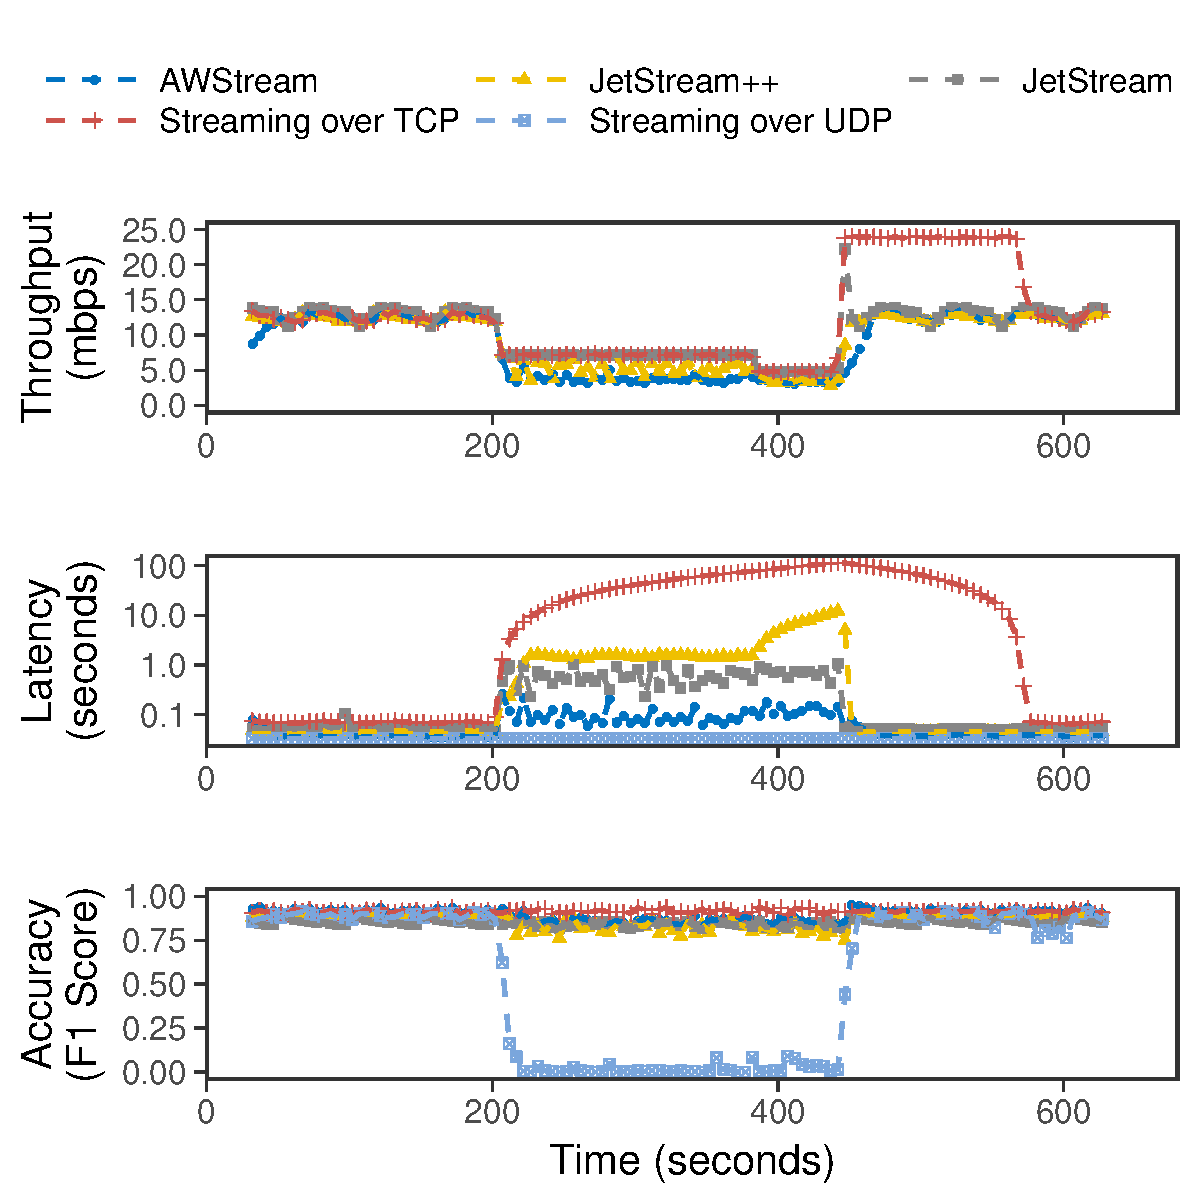
\includegraphics[width=\columnwidth]{figures/runtime_mot-timeseries.pdf}
    \caption{PD's runtime behavior with a time-series plot: throughput (top),
      showing the effect of bandwidth shaping; latency (middle) in log scale;
      and accuracy (bottom).}
    \label{fig:pd-runtime-timeseries}
  \end{subfigure}
  \vspace{1em}
  \\
  \begin{subfigure}[t]{\columnwidth}
    \centering
    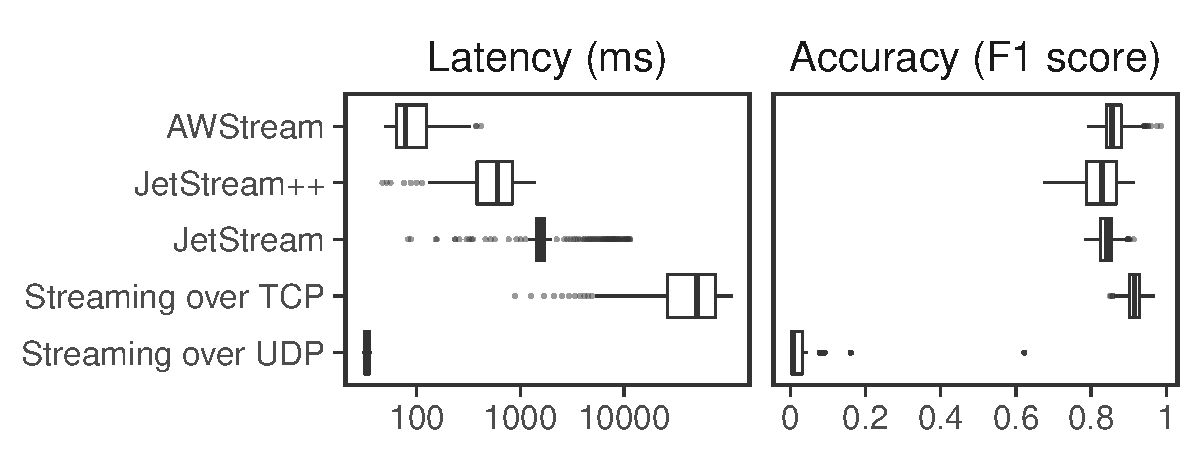
\includegraphics[width=\columnwidth]{figures/runtime_mot-boxplot.pdf}
    \caption{PD's performance summary of latency and accuracy during the traffic
      shaping (between t=200s and t=440s).}
    \label{fig:pd-runtime-boxplot}
  \end{subfigure}
  \caption{PD runtime evaluation.}
  \label{fig:pd-runtime}
  \vspace{-0.5em}
\end{figure}

\begin{figure}[t]
  \begin{subfigure}[t]{\columnwidth}
    \centering
    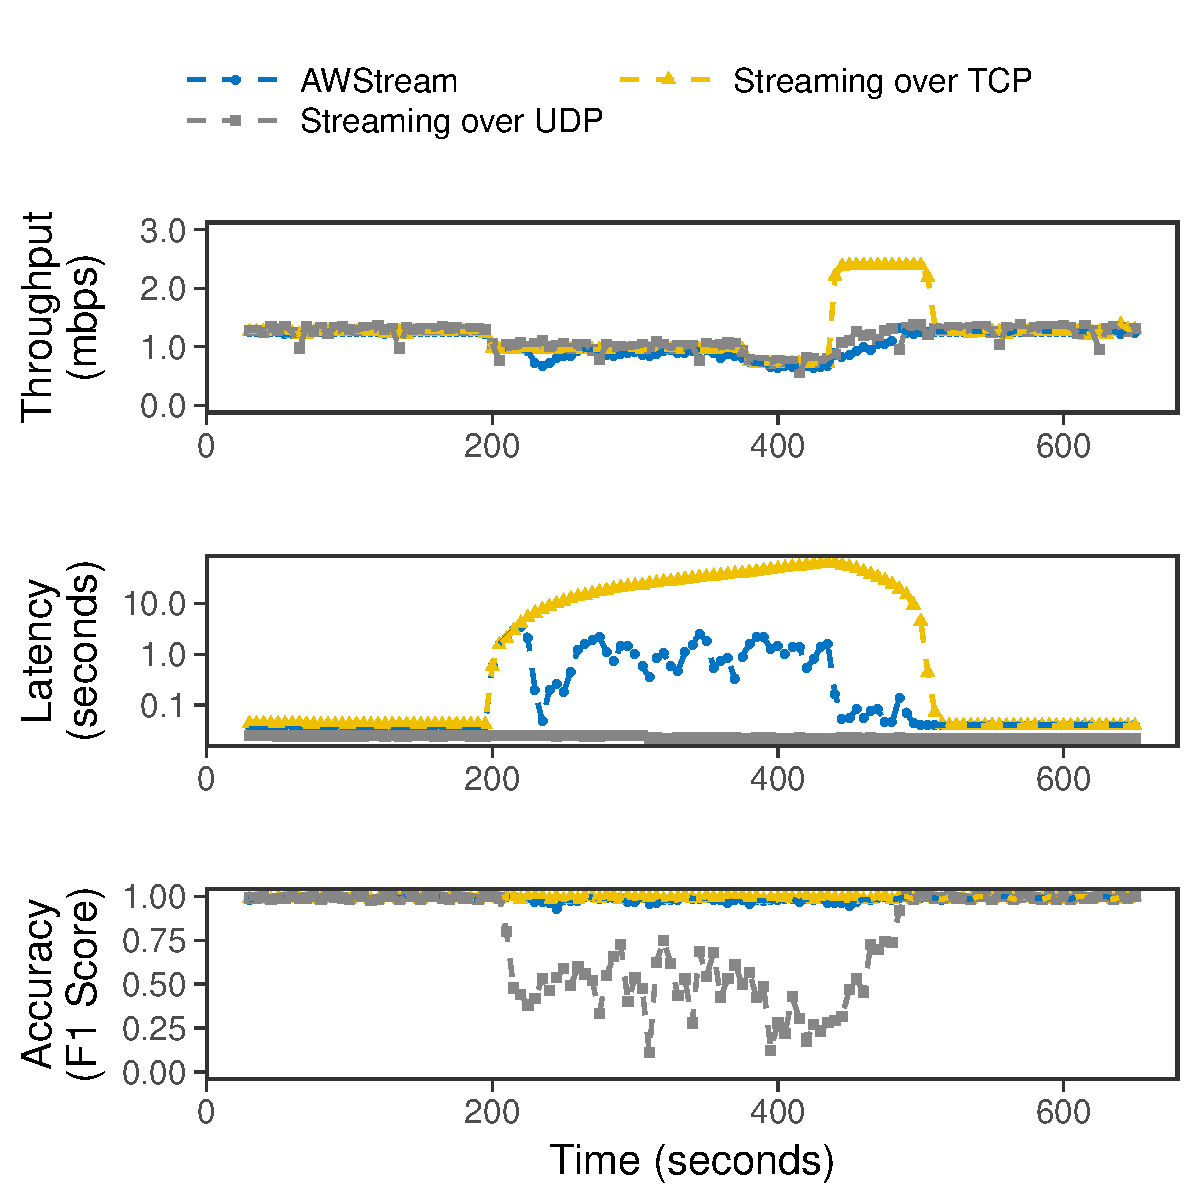
\includegraphics[width=\columnwidth]{figures/runtime_tk-timeseries.pdf}
    \caption{TK's runtime behavior with a time-series plot: throughput (top),
      showing the effect of bandwidth shaping; latency (middle) in log scale;
      and accuracy (bottom).}
    \label{fig:tk-runtime-timeseries}
  \end{subfigure}
  \vspace{1em}
  \\
  \begin{subfigure}[t]{\columnwidth}
    \centering
    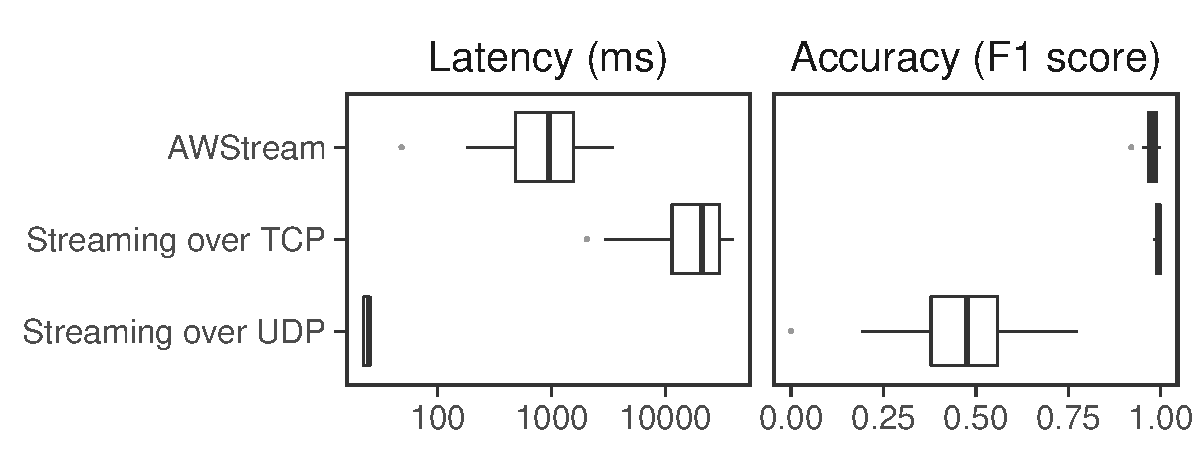
\includegraphics[width=\columnwidth]{figures/runtime_tk-boxplot.pdf}
    \caption{TK's performance summary of latency and accuracy during the traffic
      shaping (between t=200s and t=440s).}
    \label{fig:tk-runtime-boxplot}
  \end{subfigure}
  \caption{TK runtime evaluation.}
  \label{fig:tk-runtime}
  \vspace{-0.5em}
\end{figure}

\paraf{Pedestrian Detection.} The setup for PD is the same with AR: three Amazon
EC2 as clients and one as server. The maximal configuration $c_{\max}$ is
1920x1080 resolution, \(10~\text{FPS}\) and a quantization of 20; it consumes
about \SI{12}{Mbps}. For PD, \sysname{} learns that frame rate is less important
than resolution. It favors 10FPS with 1080p instead of 30FPS with 900p as in AR.

When running experiments, we use the same bandwidth shaping schedule as we used
for AR. Baselines are also the same: Streaming over TCP, streaming over UDP,
JetStream, JetStream++, and HLS.

\autoref{fig:pd-runtime} shows the runtime behavior in both time series
(throughout the experiment) and box plot (between t=200s and t=440s).  Most
observations we made in the main paper are the same here: $(i)$~Streaming with
TCP has the highest accuracy (median 92\%) at a cost of high
latency. $(ii)$~Streaming with UDP has the lowest bounded latency but the
accuracy is too low. $(iii)$~HLS incurs a latency of 2-3 seconds due to
chunking, buffering, and client fetching; its accuracy in PD is quite poor
because HLS reduces latency and encoding quality. $(iv)$~JetStream and
JetStream++ can balance latency and accuracy; but JetStream's manual policy is
unable to sustain \SI{5}{Mps} bandwidth, so its median latency is high
(\SI{1535}{\ms}); JetStream++'s latency is lower (\SI{598}{\ms}) than JetStream,
but its accuracy (82\%) suffers from policy oscillation. \sysname{} is able to
achieve the lowest latency (\SI{78}{ms}) with small accuracy drop (86\%, 6\%
drop in comparison to TCP). In comparison to the state-of-the-art system
JetStream, \sysname{} improves the latency by 20$\times$ (from \SI{1535}{ms} to
\SI{78}{ms}) and accuracy by 1\% (from 84\% to 85\%).

\para{Top-K.} For TK, our logs are split into four groups. We then use four
Amazon EC2 as clients and one as server. The maximal configuration $c_{\max}$ is
$N=9750$ for \texttt{head} and $T=0$ for \texttt{threshold}; it consumes about
\SI{1.2}{Mbps}. Because the overall bandwidth consumption is much smaller than
video analytics, we change the bandwidth parameter for runtime evaluation:
during t=200-380s, we limit the bandwidth to \SI{750}{Kbps}; during t=380-440s,
the bandwidth is \SI{500}{Kbps}; the background limit is \SI{2.5}{Mpbs}.

We've only compared \sysname{} with two baselines: streaming over TCP and
streaming over UDP. For TCP baseline, we use \sysname{} but disable the
adaptation. For UDP baseline, we implemented a simple application
protocol---packetization and a custom header---so that the receiver can still
aggregate data in the presence of UDP packet loss. While JetStream provides a
Top-K implementation, it is based on Three-Phase Uniform Threshold (TPUT) and
not suitable for low-latency Top-K monitoring. We quote from the original paper
of TPUT~\cite{cao2004efficient}, \textit{``in our target environments the query
  is asked hourly or daily. The intervals between the queries are typically long
  enough that the top-k objects have changed completely.''} In addition, we did
not implement our Top-K pipeline (\autoref{fig:topk}) with JetStream because
video analytical applications suffice the purpose of comparison.

\autoref{fig:tk-runtime} shows the evaluation results for the Top-K
application. Streaming over TCP has the highest accuracy (\textasciitilde
99.7\%) but the worst latency (up to 40 seconds). Streaming over UDP has the
lowest latency but its accuracy is the worst (\textasciitilde 52\%). \sysname{}
achieves low latency (\textasciitilde 1.1 second) and high accuracy
(\textasciitilde 98\%) simultaneously. Notice that because TK's source generates
data every second after the \texttt{Window} operation, one object in the queue
leads to one second latency. \sysname{} manages to avoid queues for most times.

\subsection{Performance with Various Network Delays}
\label{sec:various-rtt}

\sysname{} targets at wide area whose key characteristic is the large variation
in latency~\cite{li2010cloudcmp}. While we've conducted experiments using
real-world setup on Amazon EC2, the latency between EC2 sites is relatively low.
To evaluate how \sysname{} performs with increased network delays, we conducted
another experiment with one pair of client and server under different network
conditions. We use \texttt{netem} to add delays in addition to our bandwidth
shaping. The additional one-way delays ranges from 0 to \SI{250}{ms}, following
a normal distribution where the variation is 10\% of the added delay, e.g.
$250\pm 25\text{ms}$. We add delays in both direction, so the added RTT can be
as high as \SI{500}{ms}.

\begin{figure}
  \centering
  \includegraphics[width=.88\columnwidth]{figures/runtime_darknet-bench.pdf}
  \vspace{-0.5em}
  \caption{\sysname{} maintains low latency and high accuracy under different
    network delay conditions.}
  \label{fig:ar-rtt}
  \vspace{-0.5em}
\end{figure}

\autoref{fig:ar-rtt} shows the runtime behavior with various added network
delays. While the latency increases with the added delay, \sysname{} mostly
manages to achieve sub-second latency for all conditions. We see a higher
variation in latency and more outliers as network delay increases. This is
caused by a slow congestion detection when the RTT is high. In terms of
accuracy, because \sysname{} mostly stays in \texttt{Steady} state and accuracy
only depends on the level of degradation, \sysname{} achieves similar accuracy
for different network delays.

\subsection{Resource Allocation and Fairness}
\label{sec:multi-task-alloc}

\begin{figure}
  \centering
  \begin{subfigure}[t]{0.7\columnwidth}
    \centering
    
\includegraphics[width=\textwidth]{figures/multitask-legend.pdf}
  \end{subfigure}
  \\
  \vspace{0.4em}
  \begin{subfigure}[t]{0.45\columnwidth}
    \centering
    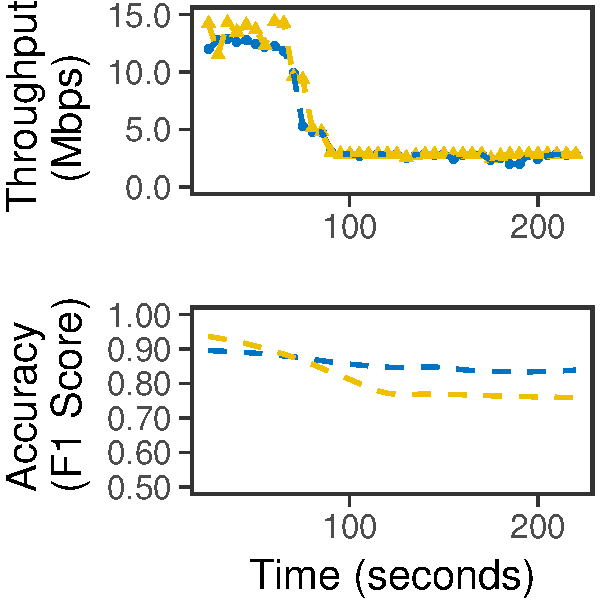
\includegraphics[width=\textwidth]{figures/multitask-left.pdf}
    \caption{Resource Fairness}
    \label{fig:eq-bw}
  \end{subfigure}
  \hfill
  \begin{subfigure}[t]{0.45\columnwidth}
    \centering
    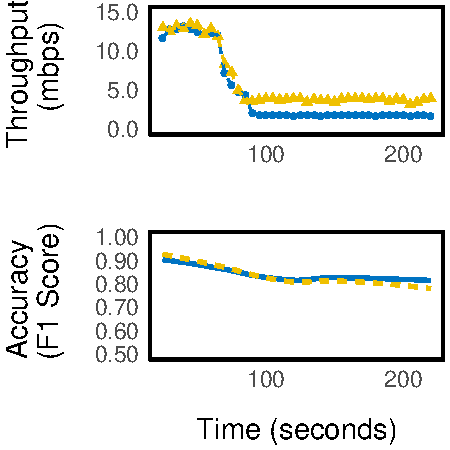
\includegraphics[width=\textwidth]{figures/multitask-right.pdf}
    \caption{Utility Fairness}
    \label{fig:eq-acc}
  \end{subfigure}
  \caption{\sysname{} supports a variety of resource allocation schemes:
    resource fairness (a) and utility fairness (b).}
  \label{fig:multitask}
  \vspace{-0.5em}
\end{figure}

We evaluate resource allocations with two applications. In this way, the result
also covers the case of a single application, and can generalize to more
applications.

We choose AR and PD as the example applications.  The clients and servers of
both applications are co-located so that they share the same bottleneck
link. The experiment starts with sufficient bandwidth. At t=60s, we start
traffic shaping to limit the total bandwidth to \SI{6}{Mbps}. When we allocate
resource equally between two applications (\autoref{fig:eq-bw}), each
application gets \SI{3}{Mbps}. Under this condition, PD runs with a higher
accuracy of 85\% while AR only achieves 77\%. In addition to resource fairness,
\sysname{} supports utility fairness: it chooses configurations that maximize
the minimal accuracy. In this experiment, PD receives \SI{2}{Mbps} and AR
receives \SI{4}{Mbps}; and both achieve 80\% accuracy (\autoref{fig:eq-acc}).

%%% Local Variables:
%%% mode: latex
%%% TeX-master: "../awstream"
%%% End:

%% LocalWords: TK PD runtime JetStream AR alloc YOLO dataset outliers
%% LocalWords: makespan subsec mins tcp boxplot geo HLS ffmpeg geforce
%% LocalWords: HLS PD's mis bw quantization RTSP RTP GPUs parallelization
%% LocalWords: eq netem resizes RTTs parallelize LFS UDP GTX analytics
%% LocalWords: FFmpeg GeForce HLS's JetStream's TK's
\section{Related Work}
\label{sec:related-work}

The work most closely related to \sysname{} is
JetStream~\cite{rabkin2014aggregation}. Both systems target at wide-area
streaming analytics. JetStream proposes to use aggregation and \textit{manual}
degradation policies to achieve responsiveness in the presence of bandwidth
fluctuation. We've discussed its limitations in \autoref{sec:motivation}.

We divide other related works into stream processing systems, approximate
analytics, WAN-aware systems and adaptive video streaming.

\paraf{Stream processing systems:} Streaming databases, such as
Borealis~\cite{abadi2005design},
TelegraphCQ~\cite{chandrasekaran2003telegraphcq}, are the early academic
explorations. They pioneered the usage of dataflow models with specialized
operators for stream processing. Recent research projects and open-source
systems, such as MillWheel~\cite{akidau2013millwheel},
Storm~\cite{toshniwal2014storm}, Heron~\cite{sanjeev2015twitter}, Spark
Streaming~\cite{zaharia2013discretized}, Apache Flink~\cite{carbone2015apache},
primary focus on fault-tolerant streaming in the context of a single
cluster. While our work has a large debt to the prior streaming work, \sysname{}
is designed for the wide area and explicitly trades data fidelity for data
freshness. In contrast, these stream processing systems often choose to throttle
the source when backpressure happens.

\para{Approximate analytics:} The idea of degrading computation fidelity for
responsiveness has also been explored in other contexts. For SQL queries, online
aggregation~\cite{hellerstein1997online}, BlinkDB~\cite{agarwal2013blinkdb} and
GRASS~\cite{ananthanarayanan2014grass} speed up queries with partial data based
on a statistical model of SQL operators. For real-time processing,
MEANTIME~\cite{farrell2016meantime} uses approximation to guarantee satisfying
real-time deadlines. For video processing, VideoStorm~\cite{zhang2017live}
optimizes video stream \textit{processing} within lager clusters with
approximation and delay-tolerance for resource management and allocation. The
trade-off between available resource and application accuracy is a common theme
among all these works. \sysname{} targets at wide-area streaming analytics, an
emerging application domain especially with the advent of IoT.

\para{WAN-aware systems:} The main challenge in designing geo-distributed
systems is to cope with high latency and limited bandwidth. While some research
projects, such as Vivace~\cite{cho2012surviving}, assume the network can
prioritize a small amount of critical data to avoid delays even under
congestion, most systems reduce data transfer in the first place to avoid
congestion. For example, LBFS~\cite{muthitacharoen2001low} exploits similarities
between files or versions of the same file. Over the past few years, we have
seen a plethora of geo-distributed analytical frameworks:
WANalytics~\cite{vulimiri2015wananlytics}, Geode~\cite{vulimiri2015global},
Iridium~\cite{pu2015low}, Pixida~\cite{kloudas2015pixida},
Clarinet~\cite{viswanathan2016clarinet}, etc. They minimize data movement by
incorporating heterogeneous wide-area bandwidth information into query
optimization and data/task placement. While effective in improving analytics
efficiency, they focus on batch analytics such as MapReduce tasks or SQL
query. Such tasks are often executed once, with little real time constrain. In
contrast, \sysname{} focuses on streaming analytics that process streams of data
continuously in real time.

%% - Pixida~\cite{kloudas2015pixida} minimizes data movement across inter-DC
%% links by solving a traffic minimization problem in data analytics.

%% - Iridium~\cite{pu2015low} optimizes data and task placement jointly to
%% achieve an overall low latency goal.

%% - Clarinet~\cite{viswanathan2016clarinet} incorporate bandwidth information
%% into query optimizer to reduce data transfer.

%% WheelFS~\cite{stribling2009flexible}

%% Geode~\cite{vulimiri2015global} develops input data movement and join
%% algorithm selection strategies to minimize WAN bandwidth usage.

%% WANalytics~\cite{vulimiri2015wananlytics} focuses on batch analytics.

%% SWAG~\cite{hung2015scheduling} coordinates compute task scheduling across
%% DCs.

%% \cite{heintz2015towards} discusses the complex tradeoffs involved in
%% wide-area analytics.

\para{Adaptive video streaming:} Designing a good adaptation strategy to improve
QoE for video streaming has been a hot topic. Research
projects~\cite{yin2015control, sun2016cs2p} and industrial efforts
HLS~\cite{pantos2016http}, DASH~\cite{sodagar2011mpeg,
  michalos2012dynamic}. Despite fruitful, their results are not directly
transferable to the wide-area streaming analytics. \sysname{} attempts at a
generalization with \maybe{} APIs to allows more custom control over what
parameters can be adjusted. \sysname{} is not competing with video streaming
technologies. Instead, our APIs are extensible to incorporate techniques such as
video encoding (H.264~\cite{richardson2011h} or VP9~\cite{grange2016vp9}). The
main contribution of \sysname{} here is to provide a system for arbitrary
streaming analytics to benefit from adaptation.

%% TCP, for example, adapts to available bandwidth by controlling the congestion
%% window with AIMD~\cite{jacobson1988congestion}.  Previous work has proposed
%% modifications to TCP for specific contexts. For streaming over TCP, Goel et
%% al.~\cite{goel2008low} proposes adaptive buffer-size tuning. For the cloud,
%% Adaptive TCP~\cite{wu2013adaptive} proposes to modify the congestion control
%% behavior based on flow size for the cloud.

% \para{Scheduling and allocation:} Resource allocations in the cloud is how to
% efficiently allocate tasks.  In the wide area, we face fundamental limit that
% therefore degradation is more effective. For multiple tasks, Existing
% allocations are for resources without considering application trade-offs.
% MediaNet~\cite{hicks2003user} uses both local and online global resource
% scheduling to improve user performance and network utilization, and adapts
% without requiring underlying support for resource
% reservations. VideoStorm~\cite{zhang2017live} primarily focuses on cluster
% resource allocation among video queries. For wide-area, the resource
% allocation is limited. We do not control the capacity; but still we can
% allocate the available bandwidth.

% Performance modeling: CherryPick~\cite{alipourfard2017cherrypick},
% Ernest~\cite{venkataraman2016ernest}.
%% Dolly~\cite{ananthanarayanan2013effective}.
%% \para{Program Synthesis:}

%%% Local Variables:
%%% mode: latex
%%% TeX-master: "sosp17"
%%% End:


{\bibliographystyle{acm}\bibliography{sigcomm2017}}

\end{document}

%%% Local Variables:
%%% mode: latex
%%% TeX-master: t
%%% End:
